%%%  کلاس AUTthesis، نسخه آبان 1397
%%%   دانشگاه صنعتی امیرکبیر                 http://www.aut.ac.ir
%%%  تالار گفتگوی پارسی‌لاتک،       http://forum.parsilatex.com
%%%   آپدیت شده در آبان 95
%%%   پشتیبانی و راهنمایی          badali_farhad@yahoo.com
%%%
%%%   بازبینی و اصلاح شده در آبان ماه 1397
%%%  Tested via TeXstudio in TeXlive 2014-2018.
%%%

%-----------------------------------------------------------------------------------------------------
%        روش اجرا.: 2 بار F1 ، 2 بار  F11(به منظور تولید مراجع) ، دوبار Ctrl+Alt+I (به منظور تولید نمایه) و دو بار F1 -------> مشاهده Pdf
%%%%%%%%%%%%%%%%%%%%%%%%%%%%%%%%%%%%%%%%%%%%%%%%%%%%%%
%   TeXstudio as your IDE
%%  برای compile در TeXstudio تنها کافی است منوی Options->Configure TeXstudio را زده و در پنجره Configure TeXstudio در بخش Build گزینه Default Compiler را به XeLaTeX تغییر دهید. سند شما به راحتی compile خواهد شد.
%   F1 & F5 : Build & view
%   F6      : Compile
%   F7      : View
%   --------------
%%%%%%%%%%%%%%%%%%%%%%%%%%%%%%%%%%%%%%%%%%%%%%%%%%%%%%
%        اگر قصد نوشتن رساله دکتری را دارید، در خط زیر به جای msc،
%      کلمه phd را قرار دهید. کلیه تنظیمات لازم، به طور خودکار، اعمال می‌شود.
%%% !TEX TS-program = XeLaTeX
\documentclass[oneside,bsc,12pt]{AUTthesis}
%       فایل commands.tex را حتماً به دقت مطالعه کنید؛ چون دستورات مربوط به فراخوانی بسته زی‌پرشین 
%       و دیگر بسته‌ها و ... در این فایل قرار دارد و بهتر است که با نحوه استفاده از آنها آشنا شوید. توجه شود برای نسخه نهایی پایان‌نامه حتماً hyperref را 
%        غیرفعال کنید.


% در این فایل، دستورها و تنظیمات مورد نیاز، آورده شده است.
%-------------------------------------------------------------------------------------------------------------------
% در ورژن جدید زی‌پرشین برای تایپ متن‌های ریاضی، این سه بسته، حتماً باید فراخوانی شود.
\usepackage{amsthm,amssymb,amsmath,amsfonts}
% بسته‌ای برای تنطیم حاشیه‌های بالا، پایین، چپ و راست صفحه
\usepackage[top=30mm, bottom=30mm, left=25mm, right=30mm]{geometry}
% بسته‌‌ای برای ظاهر شدن شکل‌ها و تصاویر متن
\usepackage{graphicx}
\usepackage{color}
%بسته‌ای برای تنظیم فاصله عمودی خط‌های متن
\usepackage{setspace}
\usepackage{titletoc}
\usepackage{tocloft}
%با فعال کردن بسته زیر فوت‌نوت‌ها در هر صفحه ریست می‌شوند. حالت پیش‌فرض آن ریست شدن در هر فصل می‌باشد.
%\usepackage[perpage]{footmisc}
\usepackage{enumitem}
%\usepackage{titlesec}
% بسته‌ و دستوراتی برای ایجاد لینک‌های رنگی با امکان جهش
\usepackage[pagebackref=false,colorlinks,linkcolor=blue,citecolor=red]{hyperref}
\usepackage[nameinlink]{cleveref}%capitalize,,noabbrev
 \AtBeginDocument{%
    \crefname{equation}{برابری}{equations}%
    \crefname{chapter}{فصل}{chapters}%
    \crefname{section}{بخش}{sections}%
    \crefname{appendix}{پیوست}{appendices}%
    \crefname{enumi}{مورد}{items}%
    \crefname{footnote}{زیرنویس}{footnotes}%
    \crefname{figure}{شکل}{figures}%
    \crefname{table}{جدول}{tables}%
    \crefname{theorem}{قضیه}{theorems}%
    \crefname{lemma}{لم}{lemmas}%
    \crefname{corollary}{نتیجه}{corollaries}%
    \crefname{proposition}{گزاره}{propositions}%
    \crefname{definition}{تعریف}{definitions}%
    \crefname{result}{نتیجه}{results}%
    \crefname{example}{مثال}{examples}%
    \crefname{remark}{نکته}{remarks}%
    \crefname{note}{یادداشت}{notes}%
}
% چنانچه قصد پرینت گرفتن نوشته خود را دارید، خط بالا را غیرفعال و  از دستور زیر استفاده کنید چون در صورت استفاده از دستور زیر‌‌، 
% لینک‌ها به رنگ سیاه ظاهر خواهند شد که برای پرینت گرفتن، مناسب‌تر است
%\usepackage[pagebackref=false]{hyperref}
% بسته‌ لازم برای تنظیم سربرگ‌ها
\usepackage{fancyhdr}
% بسته‌ای برای ظاهر شدن «مراجع»  در فهرست مطالب
\usepackage[nottoc]{tocbibind}
% دستورات مربوط به ایجاد نمایه
\usepackage{makeidx,multicol}
\setlength{\columnsep}{1.5cm}

%%%%%%%%%%%%%%%%%%%%%%%%%%
\usepackage{verbatim}
\makeindex
\usepackage{sectsty}
% فراخوانی بسته زی‌پرشین و تعریف قلم فارسی و انگلیسی
\usepackage{xepersian}%[extrafootnotefeatures]
\SepMark{-}
%حتماً از تک لایو 2014 استفاده کنید.
\settextfont[Scale=1.2]{B Nazanin}
\setlatintextfont{Times New Roman}
\renewcommand{\labelitemi}{$\bullet$}
%%%%%%%%%%%%%%%%%%%%%%%%%%
% چنانچه می‌خواهید اعداد در فرمول‌ها، انگلیسی باشد، خط زیر را غیرفعال کنید.
%در غیر اینصورت حتماً فونت PGaramond را نصب کنید.
\setdigitfont[Scale=1.1]{PGaramond}%%Yas
%%%%%%%%%%%%%%%%%%%%%%%%%%
% تعریف قلم‌های فارسی اضافی برای استفاده در بعضی از قسمت‌های متن
\defpersianfont\nastaliq[Scale=2]{IranNastaliq}
\defpersianfont\chapternumber[Scale=3]{B Nazanin}
%\chapterfont{\centering}%
%%%%%%%%%%%%%%%%%%%%%%%%%%
% دستوری برای تغییر نام کلمه «اثبات» به «برهان»
\renewcommand\proofname{\textbf{برهان}}

% دستوری برای تغییر نام کلمه «کتاب‌نامه» به «منابع و مراجع«
\renewcommand{\bibname}{منابع و مراجع}


% Headings for every page of ToC, LoF and Lot
\setlength{\cftbeforetoctitleskip}{-1.2em}
\setlength{\cftbeforelottitleskip}{-1.2em}
\setlength{\cftbeforeloftitleskip}{-1.2em}
\setlength{\cftaftertoctitleskip}{-1em}
\setlength{\cftafterlottitleskip}{-1em}
\setlength{\cftafterloftitleskip}{-1em}
%%\makeatletter
%%%%\renewcommand{\l@chapter}{\@dottedtocline{1}{1em\bfseries}{1em}}
%%%%\renewcommand{\l@section}{\@dottedtocline{2}{2em}{2em}}
%%%%\renewcommand{\l@subsection}{\@dottedtocline{3}{3em}{3em}}
%%%%\renewcommand{\l@subsubsection}{\@dottedtocline{4}{4em}{4em}}
%%%%\makeatother


\newcommand\tocheading{\par عنوان\hfill صفحه \par}
\newcommand\lofheading{\hspace*{.5cm}\figurename\hfill صفحه \par}
\newcommand\lotheading{\hspace*{.5cm}\tablename\hfill صفحه \par}

\renewcommand{\cftchapleader}{\cftdotfill{\cftdotsep}}
\renewcommand{\cfttoctitlefont}{\hspace*{\fill}\LARGE\bfseries}%\Large
\renewcommand{\cftaftertoctitle}{\hspace*{\fill}}
\renewcommand{\cftlottitlefont}{\hspace*{\fill}\LARGE\bfseries}%\Large
\renewcommand{\cftafterlottitle}{\hspace*{\fill}}
\renewcommand{\cftloftitlefont}{\hspace*{\fill}\LARGE\bfseries}
\renewcommand{\cftafterloftitle}{\hspace*{\fill}}

%%%%%%%%%%%%%%%%%%%%%%%%%%
% تعریف و نحوه ظاهر شدن عنوان قضیه‌ها، تعریف‌ها، مثال‌ها و ...
%برای شماره گذاری سه تایی قضیه ها
\theoremstyle{definition}
\newtheorem{definition}{تعریف}[section]
\newtheorem{remark}[definition]{نکته}
\newtheorem{note}[definition]{یادداشت}
\newtheorem{example}[definition]{نمونه}
\newtheorem{question}[definition]{سوال}
\newtheorem{remember}[definition]{یاداوری}
\theoremstyle{theorem}
\newtheorem{theorem}[definition]{قضیه}
\newtheorem{lemma}[definition]{لم}
\newtheorem{proposition}[definition]{گزاره}
\newtheorem{corollary}[definition]{نتیجه}
%%%%%%%%%%%%%%%%%%%%%%%%
%%%%%%%%%%%%%%%%%%%
%%% برای شماره گذاری چهارتایی قضیه ها و ...
%%\newtheorem{definition1}[subsubsection]{تعریف}
%%\newtheorem{theorem1}[subsubsection]{قضیه}
%%\newtheorem{lemma1}[subsubsection]{لم}
%%\newtheorem{proposition1}[subsubsection]{گزاره}
%%\newtheorem{corollary1}[subsubsection]{نتیجه}
%%\newtheorem{remark1}[subsubsection]{نکته}
%%\newtheorem{example1}[subsubsection]{مثال}
%%\newtheorem{question1}[subsubsection]{سوال}

%%%%%%%%%%%%%%%%%%%%%%%%%%%%

% دستورهایی برای سفارشی کردن صفحات اول فصل‌ها
\makeatletter
\newcommand\mycustomraggedright{%
 \if@RTL\raggedleft%
 \else\raggedright%
 \fi}
\def\@makechapterhead#1{%
\thispagestyle{style1}
\vspace*{20\p@}%
{\parindent \z@ \mycustomraggedright
\ifnum \c@secnumdepth >\m@ne
\if@mainmatter

\bfseries{\Huge \@chapapp}\small\space {\chapternumber\thechapter}
\par\nobreak
\vskip 0\p@
\fi
\fi
\interlinepenalty\@M 
\Huge \bfseries #1\par\nobreak
\vskip 120\p@

}

%\thispagestyle{empty}
\newpage}
\bidi@patchcmd{\@makechapterhead}{\thechapter}{\tartibi{chapter}}{}{}
\bidi@patchcmd{\chaptermark}{\thechapter}{\tartibi{chapter}}{}{}
\makeatother

\pagestyle{fancy}
\renewcommand{\chaptermark}[1]{\markboth{\chaptername~\tartibi{chapter}: #1}{}}

\fancypagestyle{style1}{
\fancyhf{} 
\fancyfoot[c]{\thepage}
\fancyhead[R]{\leftmark}%
\renewcommand{\headrulewidth}{1.2pt}
}


\fancypagestyle{style2}{
\fancyhf{}
\fancyhead[R]{چکیده}
\fancyfoot[C]{\thepage{}}
\renewcommand{\headrulewidth}{1.2pt}
}

\fancypagestyle{style3}{%
  \fancyhf{}%
  \fancyhead[R]{فهرست نمادها}
  \fancyfoot[C]{\thepage}%
  \renewcommand{\headrulewidth}{1.2pt}%
}

\fancypagestyle{style4}{%
  \fancyhf{}%
  \fancyhead[R]{فهرست جداول}
  \fancyfoot[C]{\thepage}%
  \renewcommand{\headrulewidth}{1.2pt}%
}

\fancypagestyle{style5}{%
  \fancyhf{}%
  \fancyhead[R]{فهرست اشکال}
  \fancyfoot[C]{\thepage}%
  \renewcommand{\headrulewidth}{1.2pt}%
}

\fancypagestyle{style6}{%
  \fancyhf{}%
  \fancyhead[R]{فهرست مطالب}
  \fancyfoot[C]{\thepage}%
  \renewcommand{\headrulewidth}{1.2pt}%
}

\fancypagestyle{style7}{%
  \fancyhf{}%
  \fancyhead[R]{نمایه}
  \fancyfoot[C]{\thepage}%
  \renewcommand{\headrulewidth}{1.2pt}%
}

\fancypagestyle{style8}{%
  \fancyhf{}%
  \fancyhead[R]{منابع و مراجع}
  \fancyfoot[C]{\thepage}%
  \renewcommand{\headrulewidth}{1.2pt}%
}
\fancypagestyle{style9}{%
  \fancyhf{}%
  \fancyhead[R]{واژه‌نامه‌ی فارسی به انگلیسی}
  \fancyfoot[C]{\thepage}%
  \renewcommand{\headrulewidth}{1.2pt}%
}
%


%دستور حذف نام لیست تصاویر و لیست جداول از فهرست مطالب
\newcommand*{\BeginNoToc}{%
  \addtocontents{toc}{%
    \edef\protect\SavedTocDepth{\protect\the\protect\value{tocdepth}}%
  }%
  \addtocontents{toc}{%
    \protect\setcounter{tocdepth}{-10}%
  }%
}
\newcommand*{\EndNoToc}{%
  \addtocontents{toc}{%
    \protect\setcounter{tocdepth}{\protect\SavedTocDepth}%
  }%
}
\newcounter{savepage}
\renewcommand{\listfigurename}{فهرست اشکال}
\renewcommand{\listtablename}{فهرست جداول}
%\renewcommand\cftsecleader{\cftdotfill{\cftdotsep}}
%%%%%%%%%%%%%%%%%%%%%%%%%%%%%
%%%%%%%%%%%%%%%%%%%%%%%%%%%%

\begin{document}
\baselineskip=.75cm
\linespread{1.75}
%% -!TEX root = AUTthesis.tex
% در این فایل، عنوان پایان‌نامه، مشخصات خود، متن تقدیمی‌، ستایش، سپاس‌گزاری و چکیده پایان‌نامه را به فارسی، وارد کنید.
% توجه داشته باشید که جدول حاوی مشخصات پروژه/پایان‌نامه/رساله و همچنین، مشخصات داخل آن، به طور خودکار، درج می‌شود.
%%%%%%%%%%%%%%%%%%%%%%%%%%%%%%%%%%%%
% دانشکده، آموزشکده و یا پژوهشکده  خود را وارد کنید
\faculty{دانشکده مهندسی کامپیوتر و فناوری اطلاعات}
% گرایش و گروه آموزشی خود را وارد کنید
\department{گرایش معماری سیستم‌های کامپیوتری}
% عنوان پایان‌نامه را وارد کنید
\fatitle{طراحی و پیاده‌سازی سامانه ردیابی مبتنی بر 
	\\[.75 cm]
	اینترنت اشیا}

 
% نام استاد(ان) راهنما را وارد کنید
\firstsupervisor{دکتر بهادر بخشی}
%\secondsupervisor{استاد راهنمای دوم}
% نام استاد(دان) مشاور را وارد کنید. چنانچه استاد مشاور ندارید، دستور پایین را غیرفعال کنید.
\firstadvisor{دکتر مهدی راستی}
%\secondadvisor{استاد مشاور دوم}
% نام نویسنده را وارد کنید
\name{ ساره سلطانی نژاد}
% نام خانوادگی نویسنده را وارد کنید
\surname{}
%%%%%%%%%%%%%%%%%%%%%%%%%%%%%%%%%%
\thesisdate{خرداد
	 98}

% چکیده پایان‌نامه را وارد کنید
\fa-abstract{
در علم فناوری اطلاعات، مفهوم اينترنت اشيا به اشيايي با هويت خاص اطلاق مي‌شود كه دارای شناسه منحصر به فرد بوده و توانايي انتقال داده روی شبکه، بدون نياز به تعامل و دخالت انسان را دارند. در واقع هدف اصلي آن هوشمند سازی اشيا و فراهم آوردن بستری است كه از طريق آن،
اشيا قادر به ارسال و دريافت اطلاعات با يکديگر مي‌باشند.
\\
در سال‌های اخير فناوری اينترنت اشيا رشد چشمگيری داشته و در زمينه‌های مختلف توانسته نيازهای متعدد و پيچيده‌ای را برطرف كند. يکي از كاربردهای اينترنت اشيا در زمينه‌ی ‌‌رديابي اشيا متحرك مي‌باشد كه در حوزه‌های مختلف مانند امنيت، نظارت، حمل و نقل و ... مي‌تواند مورد استفاده قرار گيرد.
\\
سيستم موقعيت‌يابي و رديابي امکان ارائه راه‌حل‌هايي مطمئن برای تامين امنيت افراد و وسايل نقليه را فراهم آورده است و همچنين تاثير بسزايي در بهينه شدن كيفيت نظارت و مديريت ناوگان‌های حمل و نقل، حركت خودروها، افراد (کودکان و سالمندان) و يا هر شي متحرك ديگر دارد. در واقع سامانه رديابي تکنولوژی است كه امکان تعيين موقعيت دقيق و رديابي افراد، وسايل نقليه و يا هر جسم متحرك ديگر را با استفاده از متدهای مختلفي مانند
سامانه موقعيت‌ياب جهاني فراهم آورده است.
\\
در اين پروژه قصد داريم سامانه‌ای را پياده‌سازی كنيم كه بتوان توسط آن موقعيت دقيق و مسير حركت هر جسم متحرك را در رديابي كرد. در اين سيستم، هر شي مجهز به يک ماژول \lr{GPS} است كه موقعيت مکاني خود را از این طریق مشخص کرده و از طريق شبکه \lr{GPRS} به سرورهای نرم‌افزاری ارسال مي‌كند. اين اطلاعات از طريق يک برنامه كاربردی از سرور دريافت شده و به صورت گرافيکي بر روی نقشه نمايش داده مي‌شود. به اين ترتيب ميتوان مسير حركت
شي، مسيرهای پرتردد و ... را از اين اطلاعات استخر كرد.
هدف از این پروژه پياده‌سازی سامانه‌ای است كه بتوان توسط آن موقعيت دقيق، مسير حركت و مسیرهای پرتردد هر جسم متحرك را در هر زمان تعيين كرد.
}


% کلمات کلیدی پایان‌نامه را وارد کنید
\keywords{موقعیت‌یاب جهانی، اینترنت اشیا، ردیابی}
\keywords{ردیابی، سامانه موقعیت‌یاب جهانی، \lr{GSM} , \lr{GPS}، اینترنت اشیا}


\AUTtitle
%%%%%%%%%%%%%%%%%%%%%%%%%%%%%%%%%%
\vspace*{7cm}
\thispagestyle{empty}
\begin{center}

\includegraphics[height=5cm,width=12cm]{besm}
\end{center}
% تاییدیه دفاع
\newpage
\thispagestyle{empty}
%\fontsize{18pt}{19pt}\selectfont

\section*{صفحه فرم ارزیابی و تصویب پایان نامه- فرم تأیید اعضاء كميته دفاع}

\fontsize{12pt}{14pt}\selectfont
%\renewcommand{\baselinestretch}{1.5}
\vspace*{1cm}
   در این صفحه فرم دفاع یا تایید و تصویب پایان نامه موسوم به فرم کمیته دفاع- موجود در پرونده آموزشی- را قرار دهید.
\vspace*{1cm}


\subsection*{نکات مهم:}
 
\begin{itemize}
\item
	نگارش پایان نامه/رساله باید به
	{\color{red}
		زبان فارسی
	}
	و بر اساس آخرین نسخه دستورالعمل و راهنمای تدوین پایان نامه های دانشگاه صنعتی امیرکبیر باشد.(دستورالعمل و راهنمای حاضر)
\item رنگ جلد پایان نامه/رساله چاپي كارشناسي، كارشناسي ارشد و دكترا  بايد به ترتيب مشكي، طوسي و سفيد رنگ باشد.  
\item چاپ و صحافی پایان نامه/رساله بصورت
{\color{red}
	پشت و رو(دورو)
}
بلامانع است و انجام آن توصيه مي شود. 
\end{itemize}
%%%%%%%%%%%%%%%%%%%%%%%%%%%%%%%%%%%%%%%%%%%%%%%%%%%%%%%%%%%%%%%%%%%%%%%%%%%%%%%%%%%%%%%%%%%%%%%%%%
%%%%%%%%%%%%%%%%%%%%%%%%%%%%%%%%%%%%%%%%%%%%%%%%%%%%%%%%%%%%%%%%%%%%%%%%%%%%%%%%%%%%%%%%%%%%%%%%%%
\newpage
\thispagestyle{empty}
\begin{picture}(50,50)
  \put(17,0){
\includegraphics[scale=1.1]{fa-logo}}
  \put(4.5,-13){\footnotesize{دانشگاه صنعتی امیرکبیر}}
  \put(10.5,-27){\footnotesize{(پلی‌تکنیک تهران)}}
  \put(170,30){\bf{به نام خدا}}
  \put(140,-5){\Large\bf{تعهدنامه اصالت اثر}}
  \put(310,0){تاریخ: \datethesis}
\end{picture}

\vspace*{2.5cm}

اينجانب {\bf{\fname\lname}} متعهد می‌شوم که مطالب مندرج در این پایان‌نامه حاصل کار پژوهشی اینجانب تحت نظارت و راهنمایی اساتید دانشگاه صنعتی امیرکبیر بوده و به دستاوردهای دیگران که در این پژوهش از آنها استفاده شده است مطابق مقررات و روال متعارف ارجاع و در فهرست منابع و مآخذ ذکر گردیده است. این پایان‌نامه قبلاً برای احراز هیچ مدرک هم‌سطح یا بالاتر ارائه نگردیده است.

در صورت اثبات تخلف در هر زمان، مدرک تحصیلی صادر شده توسط دانشگاه از درجه اعتبار ساقط بوده و دانشگاه حق پیگیری قانونی خواهد داشت.


کلیه نتایج و حقوق حاصل از این پایان‌نامه متعلق به دانشگاه صنعتی امیرکبیر می‌باشد. هرگونه استفاده از نتایج علمی و عملی، واگذاری اطلاعات به دیگران یا چاپ و تکثیر، نسخه‌برداری، ترجمه و اقتباس از این پایان نامه بدون موافقت کتبی دانشگاه صنعتی امیرکبیر ممنوع است. 
نقل مطالب با ذکر مآخذ بلامانع است.\\
\vspace{2.5cm}


{\centerline {\bf{\fname\lname}}}
\vspace*{.2cm}
{\centerline{امضا}}
%%%%%%%%%%%%%%%%%%%%%%%%%%%%%%%%%
% چنانچه مایل به چاپ صفحات «تقدیم»، «نیایش» و «سپاس‌گزاری» در خروجی نیستید، خط‌های زیر را با گذاشتن ٪  در ابتدای آنها غیرفعال کنید.
% پایان‌نامه خود را تقدیم کنید
% نیایش خود را در فایل زیر بنویسید.
%\begin{acknowledgementpage}

\vspace{1.5cm}

{\nastaliq
{
 نويسنده پايان‌نامه، درصورت تمايل ميتواند برای سپاسگزاری پايان‌نامه خود را به شخص يا اشخاص و يا ارگان خاصی تقدیم نماید.
}}\end{acknowledgementpage}
\newpage
% سپاسگزاری را در فایل زیر بنویسید.
%%%%%%%%%%%%%%%%%%%%%%%%%%%%%%%%%%%%
\newpage\thispagestyle{empty}
% سپاس‌گزاری
{\nastaliq
سپاس‌گزاری
}
\\[2cm]

 نويسنده پايان‌نامه می‌تواند مراتب امتنان خود را نسبت به استاد راهنما و استاد مشاور و یا ديگر افرادي كه طي انجام پايان‌نامه به نحوي او را یاری و یا با او همكاری نموده‌اند ابراز دارد.














% با استفاده از دستور زیر، امضای شما، به طور خودکار، درج می‌شود.
\signature








%%%%%%%%%%%%%%%%%%%%%%%%%%%%%%%%%%%%%%%%%
%%%%%%%%%%%%%%%%%%%%%%%%%%%%%%%%%کدهای زیر را تغییر ندهید.
\newpage\clearpage

\pagestyle{style2}

\vspace*{-1cm}
\section*{\centering چکیده}
%\addcontentsline{toc}{chapter}{چکیده}
\vspace*{.5cm}
\ffa-abstract
\vspace*{2cm}


{\noindent\large\textbf{واژه‌های کلیدی:}}\par
\vspace*{.5cm}
\fkeywords
% دستور زیر برای شماره گذاری صفحات قبل از فصل اول با حروف ابجد است.
\pagenumbering{alph}
%-----------------------------------------------------------------------------
% فایل زیر دستورات مربوط به نمایش صفحات فهرست مطالب- فهرست اشکال و جداول است.
%{\pagestyle{style2}
%\tableofcontents}\newpage
%
%\listoffigures
\cleardoublepage
\pagestyle{style6}
\tableofcontents
\pagestyle{style6}
\cleardoublepage
%اگر لیست تصاویر و لیست جداول ندارید ، کدهای زیر را با گذاشتن % در ابتدای آن‌ها، غیرفعال کنید.
\BeginNoToc
%============
\addtocontents{lof}{\lofheading}% add heading to the first page in LoF
\pagestyle{style5}
\listoffigures
\thispagestyle{style5}
\cleardoublepage
%============
%\addtocontents{lot}{\lotheading}% add heading to the first page in LoT
%\thispagestyle{style4}
%\listoftables
%\thispagestyle{style4}
%============
%\cleardoublepage
%
\cleardoublepage
\setcounter{savepage}{\arabic{page}}
\mainmatter
\addtocontents{toc}{\tocheading}% add heading to the first page in ToC, after frontmatter entries
\EndNoToc
% در صورت تمایل می‌توانید با فعال کردن دستور بالا، لیست تصاویر را به  پایان‌نامه خود اضافه کنید.
%-------------------------------------------------------------------------symbols(فهرست نمادها)
% وجود لیست نمادها الزامیست.(لطفاً نمادهای خود را جایگذین نمادهای پیش‌فرض کنید.)
%%%%%%%%%%%%%

{\centering\LARGE\textbf{فهرست نمادها}\par}%

\pagenumbering{alph}
\setcounter{page}{\thesavepage}
%\setcounter{page}{6}
\vspace*{1cm}

\pagestyle{style3}
%\thispagestyle{empty}
%\addcontentsline{toc}{chapter}{فهرست نمادها}
\symb{\text{ نماد}}{مفهوم}
\\
%مقادیر بالا را تغییر ندهید
%%%%%%%%%%%%%%%%%%%%%%%%%%%%%%%%%%%%%%%%%%%%%%%%%%%%%%%%%
\symb{\mathbb{R}^n}{
فضای اقلیدسی با بعد $n$
}
\symb{\mathbb{S}^n}{
کره یکه $n$ بعدی
}
\symb{M^m}{
خمینه $m$-بعدی $M$
}
\symb{\mathfrak{X}(M)}{
جبر میدان‌های  برداری هموار روی $M$
}
\symb{\mathfrak{X}^1(M)}{
مجموعه میدان‌های برداری هموار یکه روی $(M,g)$ 
}
\symb{\Omega^p(M)}{
مجموعه $p$-فرمی‌های روی خمینه $M$
}
\symb{Q}{
اپراتور ریچی
}
\symb{\mathcal{R}}{
تانسور انحنای ریمان
}
\symb{ric}{
تانسور ریچی
}
\symb{L}{
مشتق لی
}
\symb{\Phi}{
2-فرم اساسی خمینه تماسی
}
\symb{\nabla}{
التصاق لوی-چویتای
}
\symb{\Delta}{
لاپلاسین ناهموار
}
\symb{\nabla^*}{
عملگر خودالحاق صوری القا شده از التصاق لوی-چویتای
}
\symb{g_s}{
متر ساساکی
}
\symb{\nabla}{
التصاق لوی-چویتای وابسته به متر ساساکی
}
\symb{\Delta}{
عملگر لاپلاس-بلترامی روی $p$-فرم‌ها
}

%%%%%%%%%%%%%%%%%%%%%%%%%%%%%%%%%%%%%%%

\thispagestyle{style3}
\newpage
%\pagestyle{style1}
%%%%%%%%%%%%%%%%%%%%%%%%%%%%%%%%%%%%


\pagenumbering{arabic}
\pagestyle{style1}
%--------------------------------------------------------------------------chapters(فصل ها)
\chapter{مقدمه}
مفهوم اينترنت اشيا \RTLfootnote{\lr{Internet of Things (IOT)}} به اشيايي با هويت خاص اطلاق مي‌شود كه دارای شناسه منحصر به فرد بوده و توانايي انتقال داده روی شبکه، بدون نياز به تعامل و دخالت انسان را دارند. هدف اصلي آن هوشمند سازی اشيا و فراهم آوردن بستری است كه از طريق آن اشيا قادر به ارسال و دريافت اطلاعات با يکديگر مي‌باشند. اينترنت اشيا به طور گسترده به توسعه قابليت محاسبه و ارتباطات شبکه‌ای اشيا، دستگاه‌ها، سنسورها يا هر مورد ديگری كه به طور معمول به عنوان كامپيوتر در نظر گرفته نمي‌شود، اشاره دارد. اين اشيای هوشمند دارای قابليت جمع‌آوری داده از راه دور، تحليل و مديريت آن‌ها هستند. \cite{Mukhtar2015}

اینترنت اشیا مجموعه وسيعي از سنسورها و عملگرهايي است كه شرايط مختلف محیط را اندازه‌گیری و پردازش مي‌كنند. در سال‌هاي اخير فناوري اينترنت اشيا رشد چشمگيري داشته و توانسته در زمينه‌هاي مختلف، نيازهاي متعدد و پيچيده‌اي را برطرف كند. به علت گسترش فناوري‌هاي جديد، توليد سنسورهاي هوشمند، رشد تكنولوژي‌هاي ارتباطي و پيچيده شدن نيازها، اينترنت اشيا قدرت زيادي پيدا كرده و در زمینه‌های مختلف از آن استفاده مي‌شود و باعث گسترش سيستم‌هاي هوشمند در محیط شده است. این سیستم‌ها برای اینکه بتوانند اثر مثبتی بر محیط بگذارند باید با یکدیگر در تعامل باشند. فناوري‌هاي مبتني بر اينترنت اشيا نيازمندي‌هاي متفاوتي در مقايسه با ساير فناوري‌ها دارند. به طور معمول اين سيستم‌ها حافظه، توان مصرفي و پهناي باند كمتري نسبت به ساير سيستم‌ها دارند. اكثر سيستم‌هاي هوشمند مبتني بر باتري هستند و در مكاني دوردست قرار دارند به گونه‌ای كه نمیتوان به صورت مداوم آن‌ها را شارژ كرد. در نتيجه توان مصرفي و محدوده قابل پوشش براي اين سيستم‌ها به ويژه آن‌هايي كه در سطح كلان اجرا مي‌شوند مانند كشاورزي هوشمند، شهر و خانه هوشمند و مسائل رديابي، مسئله بسيار مهمي است. پروتكل‌هاي ارتباطي بي‌سيم متعددي وجود دارد كه هر كدام ويژگی منحصر به فرد خود را دارند.

يكي از كاربردهاي مهم اينترنت اشيا، سامانه‌هاي رديابي است كه در فناوري‌هاي مختلف مورد استفاده قرار مي‌گیرد. سيستم‌هاي رديابي براي اولين بار براي صنعت حمل و نقل به وجود آمدند. از نيازهاي اساسي صاحبان اين صنعت، بررسي موقعيت وسايل نقليه است. ابتدايي‌ترين سيسبتم‌هاي ساخته شده براي يافتن موقعيت، سيسبتم‌هاي غير فعال بودند كه اطلاعات را در حافظه‌اي ذخیره مي‌كردند و دسترسي به آن‌ها تنها زماني ممكن بود كه وسيله نقليه در دسترس باشد. اين نوع سيستم‌ها براي كاربردهاي بلادرنگ مناسب نيستند چون در اين كاربردها نياز است اطلاعات بلافاصله در اختيار كاربر قرار بگيرد. براي برطرف كردن اين نياز، سيستم‌هاي فعال به وجود آمدند كه با استفاده از يک سخت‌افزار تعبيه شده در وسيله نقليه و سرور رديابي از راه دور اين امكان را فراهم مي‌كنند.


امنيت در سيستم حمل و نقل تنها به حمل و نقل عمومي منتهي نمي‌شود. بلكه از مهم‌ترین نگراني‌هاي صاحبان وسايل نقليه شخصي، اطمينان از امنيت وسيله نقليه آن‌ها است. سيستم‌هاي رديابي در پيشگيري از سرقت يا یافتن وسيله سرقت شده مي‌توانند كمک كنند. پلیس نيز با استفاده از
اطلاعاتي كه سيستم رديابي تعبیه شده در وسيله نقليه ارسال مي‌كنبد مي‌توانبد موقعيت را تشخيص
بدهد.


علاوه بر وسايل نقليه، سيستم‌هاي رديابي در كاربردهاي نظارت از راه دور و نظارت بر محیط زیست نيز نقش مهمي دارند. به عنوان مثال رديابي حيوانات، انسان‌ها و موقعيت‌يابي اشيا از كاربردهاي اين سيستم می‌باشد. در مثال نظارت بر انسان‌ها، اين سيستم براي افراد سالمند كه دارای بيماري‌هاي خاص چون آلزايمر هستند و احتمال گم كردن مسير براي آنها بالا است، يا براي امنيت كودكان مي‌تواند بسيار مفيد باشد. خانواده‌ها مي‌توانند از اين سيستم براي يافتن موقعيت سالمند يا كودك خود استفاده كنند. سيستمي كه در اين پروژه پياده‌سازي كرده‌ايم مي‌تواند در موارد مختلف مورد استفاده قرار بگيرد.


\section{معرفی سیستم ردیابی}
اینترنت اشیاء یک بستر ارتباطی جدید در جهت برقراری ارتباط بین اشیا هوشمند می‌باشد. معرفی این بستر موجب شــده اســت تا امکانات جدیدی برای حل مسائلی همچون تعیین مکان و ردیابی اشیا متحرک از حمله وسایل نقلیه در سطح یک شهر، منطقه یا کشور فراهم گردد.
اینترنت اشیا یک بستر ارتباطی جدید است که به سرعت در حال بدست آوردن راهکارهایی در رابطه با سناریوی ارتباط از راه دور می‌باشد و انتظار می‌رود که مبادله اطلاعات در رابطه با هر شی در شبکه‌های زنجیره‌ای منابع جهانی را آسان کند، شفافیت را افزایش دهد و کارایی‌شان را بالا ببرد. به طور گسترده اینترنت اشیا می‌تواند به عنوان ستون اصلی سیستم‌های فراگیر و فعال‌سازی محیط‌های هوشمند برای سادگی در تشخیص و شناسایی اشیا و بازیابی اطلاعات از اینترنت در هر زمان و در هر مکان به کار برده شود.


از یک دیدگاه مفهومی، اینترنت اشیا متکی بر سه اصل مرتبط با توانایی اشیا هوشمند است: ۱- قابلیت شناسایی (هر چیزی خود را شناسایی کند) ۲- قابلیت انتقال (هر چیزی دست به انتقال می‌زند) ۳- قابلیت تعامل (هر چیزی دست به تعامل می‌زند) یا در میان خودشان و یا با کاربران نهایی یا سایر نهادهای فعال در شبکه. اشیا معمولا یا به صورت منحصر به فردو یا به عنوان عضوی از یک رده شناسایی می‌شوند.


یکی از مساپل مطرح امروزی، ردیابی بی‌درنگ اشیا متحرک می‌باشد که به ردیابی بی‌درنگ موقعیت فعلی یک شی متحرک معین اشاره دارد. 
سیستم ردیابی اشیا متحرک یک راه‌حل برای بسیاری از مشکلات از جمله مساپل امنیتی است. تکنولوژی است که برای مشخص کردن موقعیت شی مورد استفاده قرار می‌گیرد.
   
\chapter{اینترنت اشیا‌}
\section{طریقه‌ی مرجع نویسی}

\chapter{اجزای مورد استفاده در سیستم ردیابی}
%\thispagestyle{empty}

\section{مقدمه}
هدف اصلی پروژه ما طراحی و پياده‌سازی سامانه‌ای است كه بتوان توسط آن موقعيت دقيق و مسير
حركت هر جسم متحرك را در هر زمان تعيين كرد. سامانه ذکر شده باید علاوه بر عملکرد مناسب، از لحاظ هزینه هم به صرفه باشد.


برای این که بتوانیم چنین سامانه‌ای را طراحی کنیم اول باید نیازمندی‌های سامانه را تشخیص دهیم، معماری کلی سامانه موردنظر خود را به دست آوریم و سپس با استفاده از این معماری و نیازسنجی انجام شده برای پیاده‌سازی از ماژول‌های مناسب استفاده کنیم. در این فصل در قسمت ۳-۲ ابتدا طرح کلی سامانه ردیابی را توضیح می‌دهیم و سپس در بخش ۳-۳ اجزاء مورد استفاده در این طرح را معرفی می‌کنیم.
\section{طراحی و معماری سیستم}
در اين پروژه قصد داريم به ساخت يک سيستم رديابي بپردازيم كه قادر است موقعيت دقيق و مسير حركت يک شي متحرك را مشخص كند. در انجام اين پروژه ارتباط ما به صورت يک طرفه خواهد بود به اين صورت كه به طور پيوسته مختصات مکاني شي متحرك توسط ماژول
 جی پی اس
 \RTLfootnote{\lr{GPS: Global Positioning System}}
  اندازه گرفته ميشود و به يک سرور فرستاده ميشود. اين ماژول به طور پيوسته با ماهواره برای گرفتن مختصات مکاني در ارتباط است. دادههای GPS به آردوينو فرستاده مي‌شود. در نهايت مودم GSM 3 اين اطلاعات را برای سرورهای
نرم‌افزاری ارسال مي‌كند. در اين پروژه سرورهای نرمافزاری پس از دريافت اطلاعات، آنها را تحليل ميكنند و درخواستي از سمت سرور نخواهيم داشت و ارتباط ما به صورت يکطرفه خواهد بود. در اين قسمت پروژه يک نرم‌افزار تحت وب توسعه داده خواهد شد تا
بتواند اطلاعات ارسالي را پردازش كرده و سپس آنها را در يک پايگاه داده ذخيره كند و در انتها اطلاعات ذخيره شده را به صورت قابل نمايش برای كاربران تبديل كند. هدف اصلي از انجام اين پروژه اين است كه مسير حركت شي متحرك را بر روی نقشه نشان
دهيم.
\verb;chapter1;
\section{اجزاء سیستم}
در قسمت قبل معماري سيستم را مشخص كرديم. حال اجزاء اين معماري را به طور دقيق بيان و معرفي می‌کنیم.
\subsection{اجزاء سخت‌افزاری}
اجزای سخت‌افزاری که برای پیاده‌سازی این سامانه استفاده شده است عبارتند از:
\begin{itemize}
	\item
	ماژول آردوینو
	\item
ماژول سیم ۸۰۸
\RTLfootnote{\lr{SIM 808}}
	\item
	آنتن جی پی اس
	\RTLfootnote{\lr{GPS Antenna}}
	\item
	آنتن جی اس ام
	\RTLfootnote{\lr{GSM Antenna}}
\end{itemize}
\subsection{ماژول آردوینو}
آردوينو يک ريزپردازنده متن‌باز اس كه براي نوشتن برنامه‌هايي كه با محیط و اشیا بیرون در تعامل هستند مناسب است. این برد مناسب نمونه‌سازی می‌باشد و نرم افزار و طرح سخت‌افزار آن به صورت آزاد در اختیار تمام افراد قرار گرفته است و هر فرد علاقه‌مند حتی با دانش و تجربه اندک در حوزه الکترونیک مي‌تواند از آردوینو برای انجام پروژه‌های خود استفاده نماید.


آردوينو محیط ساده‌ای براي برنامه‌نويسي دارد كه هر شخصي با اندكي آشنایی با زبان \lr{C} و  \lr{C++} مي‌تواند در این محیط برنامه‌نويسي كند و برنامه نوشته شده را در آردوینو اجرا نماید. به ميكروكنترلر آردوينو ميتوان حسگرهاي مختلف متصل و آن‌ها را كنترل كرد. ریزپردازنده به‌ کار رفته بر روی برد آردوینو بر اساس زبان برنامه‌نویسی آردوینو بر پایه \lr{Wiring} و محیط ویژه کدنویسی آن بر پایه \lr{Processing }برنامه‌ریزی شده است و برای کدنویسی به نرم‌افزار یا کامپایلر جانبی نیازی ندارد. 


آردوينو انواع مختلفي دارد كه ما از آردوینو \lr{Uno R3 } در این پروژه استفاده کرده‌ایم. \lr{R3} سومین و آخرین نسخه آردوینو \lr{Uno} می‌باشد. برد آردوینو \lr{Uno} یک میکروکنترلر بر پایه \lr{ATmega328} می‌باشد. ولتاژ كاري آن ۵ ولت مي‌باشد. ولتاژ ورودي این برد می‌تواند در بازه ۷ تا ۲۰ ولت باشد. این برد داراي ۶ پین ورودی آنالوگ، ۱۴ پين ورودي و خروجی ديجيتال، یک پورت یو اس \RTLfootnote{\lr{USB Port}}، یک ورودی منبع تغذیه و یک دکمه بازنشانی \RTLfootnote{\lr{Reset}} است که اجازه اتصال بردهای توسعه مختلفی را فراهم می‌آورد. در شكل ۳-۱ برد آردوينو \lr{Uno} را مشاهده مي‌كنيد.
\begin{figure}[!h]
	\centerline{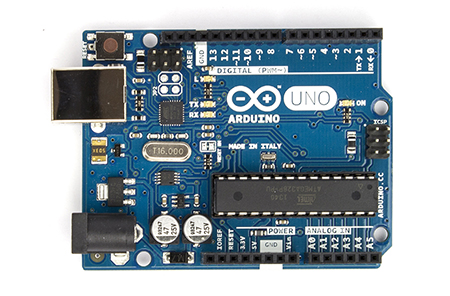
\includegraphics[width=.5\textwidth]{ArduinoUno_R3}}
	\caption{برد آردوینو \lr{UNO R3}}
\end{figure}
\subsection{ماژول \lr{SIM 808}}

ماژول \lr{SIM 808} یک ماژول ترکیبی از \lr{GSM/GPRS} و ماژول \lr{GPS}  با قابلیت پشتیبانی از چهار باند فرکانسی ۸۵۰/۹۰۰/۱۸۰۰/۱۹۰۰ مگاهرتز \RTLfootnote{\lr{MHZ}} برای ارسال داده، پیام کوتاه \RTLfootnote{\rl{SMS}} و برقراری تماس صوتی می‌باشد. این ماژول دارای یک سوکت سیم‌کارت می‌باشد که سیم‌کارت در داخل آن قرار می‌گیرد.این ماژول بر پایه آخرین ماژول \lr{GSM/GPS} از شرکت \lr{SIMCOM} می‌باشد که از شبکه چهار باند \lr{GSM|GPRS} پشتیبانی و برای ردیابی ماهواره‌ای از فناوری \lr{GPS} استفاده می‌کند. در واقع با استفاده از مودم \lr{GSM/GPRRS} و ماژول سیم ۸۰۸ می‌توان به تبادل داده روی شبکه \lr{GSM} از طریق واسط \lr{َUSB} پرداخت و از طریق به اطلاعات دستگاه‌های مستقر در مکان‌های دور دسترسی یافت.

طراحی فشرده این تراشه که دو سیستم مخابراتی و موقعیت‌یاب را در یک بسته ادغام می‌کند موجب کاهش هزینه و زمان برای انجام پروژه‌های مبتنی بر \lr{GPS} شده است. این ماژول با تکنولوژی ذخیره انرژی\lr{Power Saving} طراحی شده است و مصرف انرژی آن در حالت خواب بسیار کم در حدود یک میلی آمپر می‌باشد.
 
 
 این ماژول دارای ۶۸ پین \lr{SMT}، سوکت یو اس بی، سیم‌کارت، بلوتوث می‌باشد. دارای حساسیت بالای دریافت موقعیت جهانی با ۲۲ کانال ردیابی و ۶۶ کانال گیرنده می‌باشد. علاوه بر این از \lr{A-GPS} پشتیبانی می‌کند که برای موقعیت‌یابی داخل ساختمان استفاده می‌شود. این ماژول از طریق واسط \lr{UART} توسط فرمان \lr{AT} کنترل می‌شود و از سطح منطقی ۳.۳ تا ۵ ولت پشتیبانی می‌کند.
 از جمله ویژگی‌های این تراشه می‌توان موارد زیر را نام برد:
\begin{itemize}
	\item 
	پشتیبانی از سیم‌کارت تمامی آپراتورها
	\item
	دارای رابط \lr{SPI/USB\/Serial} و صدای آنالوگ
	\item
	دارای مدار کنترل شارژ
	\item
	پشتیبانی از فرکانس ساعت
	\item
	کم‌مصرف (۱ میلی آمپر در حالت خواب)
	\item 
	ولتاژ ورودی ۳.۴ تا ۴.۴ ولت
	\item 
	قابلیت نصب ۳ آنتن \lr{GPS, GSM, Bluetooth}
\end{itemize} 
در شکل ۳-۲ و ۳-۳ این تراشه را مشاهده می‌کنید.
\begin{figure}[!h]
	\centerline{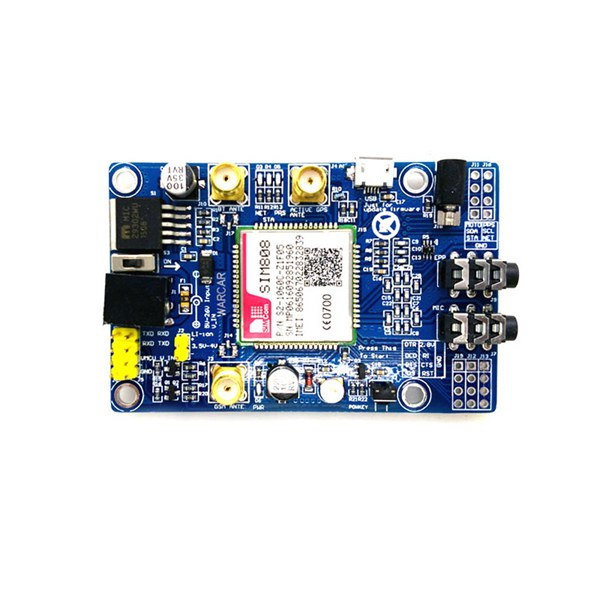
\includegraphics[width=.5\textwidth]{frontside-sim808}}
	\caption{نمایی از قسمت روبرو تراشه \lr{SIM 808}}
\end{figure}
\begin{figure}[!h]
	\centerline{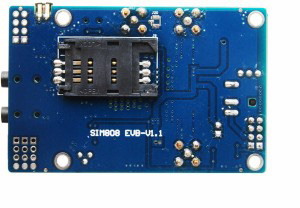
\includegraphics[width=.5\textwidth]{backside-sim808}}
	\caption{نمایی از قسمت پشت تراشه \lr{SIM 808}}
\end{figure}

\subsection{آنتن \lr{GPS}}
بهتر است قبل از معرفي آنتن \lr{GPS}، شيوه موقعيت‌يابي توسط سيستم موقعیت‌یاب جهانی \RTLfootnote{\lr{GPS}} را به طور مختصر توضيح بدهيم. سيستم \lr{GPS} در واقع شامل ۲۷ ماهواره است كه در اطراف زمين در حال گردش هستند كه از اين ۲۷ ماهواره ۳ تا به صورت رزرو شده مي‌باشند. هر ماهواره سيگنال‌هاي منحصر به فرد و پارامترهاي مداري را ارسال مي‌كند و هر گیرنده‌ای كه اين سيگنال را درياف كند، با رمزيشايي اطلاعات دريافتي مي‌تواند موقعيت دقيق ماهواره را پيدا كند. با اتصال سيستم موقعيت‌ياب به سه ماهواره مي‌توان موقعيت دوبعدي يعني طول و عرض جغرافيايي و با اتصال به چهار ماهواره ميتوان موقعيت سه بعدي را به دست آورد.


در این پروژه برای یافتن موقعیت از آنتن \lr{GPS} استفاده می‌کنیم. این ماژول قادر است موقعیت مکانی، زمان، تاریخ و سرعت را در اختیار کاربر قرار دهد. این آنتن جریان حدود ۱۰ میلی آمپر می‌کشد.
جی پی اس با دریافت سیگنال های ماهواره, موقعیت و مکان شی را مشخص میکند. برای دریافت درست سیگنال باید از آنتن استفاده شود. سیگنال های ماهواره ای جی پی اس در خطوط L1 و  L2 به ترتیب دارای فرکانس های 1575.42MHZ  و 1228MHZ می باشند.

اما قدرت سیگنال دریافتی معمولا ضعیف بوده و در حدود  166DBM میباشد. که این موضوع لزوم وجود آنتن و تقویت کننده سیگنال جی پی اس را نشان میدهد.
\subsection{اجزاء نرم‌افزاری}

\section{رعایت قواعد نشانه‌گذاری}
منظور از نشانه‌گذاري به‌کار‌بردن علامت‌ها و نشانه‌هايي است که خواندن و فهم درست یک جمله را ممکن و آسان مي‌کند. در ادامه نشانه‌هاي معمول و متداول در زبان فارسي و موارد کاربرد آنها به اختصار معرفی می‌شوند.

\subsection{ويرگول}
ويرگول نشانه ضرورت یک مکث کوتاه است و در موارد زير به‌کار مي‌رود:
\begin{itemize}
\item
در ميان دو کلمه که احتمال داده شود خواننده آنها را با کسره اضافه بخواند، يا نبودن ويرگول موجب بروز اشتباه در خواندن جمله شود.
\item
در موردي که کلمه يا عبارتي به‌‌‌‌عنوان توضيح، در ضمن یک جمله آورده شود. مثلاً برای کنترل وضعیت فضاپیماها، به‌دلیل آن‌که در خارج از جو هستند، نمی‌توان از بالک‌های آیرودینامیکی استفاده کرد.
\item
جدا‌کردن بخش‌هاي مختلف يک نشاني يا یک مرجع
\item
موارد دیگر از این قبیل
\end{itemize}
پیش از ويرگول نبايد فاصله گذاشته شود و پس از آن يک فاصله لازم است و بيشتر از آن صحیح نیست.
\subsection{نقطه}
نقطه نشانه پایان یک جمله است. پیش از نقطه نبايد فاصله گذاشته شود و پس از آن يک فاصله لازم است و بيشتر از آن صحیح نیست.
\subsection{دونقطه}
موارد کاربرد دونقطه عبارتند از:
\begin{itemize}
\item
پيش از نقل قول مستقيم
\item
پيش از بيان تفصيل مطلبي که به اجمال به آن اشاره شده‌است.
\item
پس از واژه‌اي که معني آن در برابرش آورده و نوشته مي‌شود.
\item
پس از کلمات تفسير‌کننده از قبيل «يعني» و ...
\end{itemize}
پیش از دونقطه نبايد فاصله گذاشته شود و پس از آن يک فاصله لازم است و بيشتر از آن صحیح نیست.
\subsection{گیومه}
موارد کاربرد گیومه عبارتند از:
\begin{itemize}
\item
وقتي که عين گفته يا نوشته کسي را در ضمن نوشته و مطلب خود مي‌آوريم. 
\item
در آغاز و پايان کلمات و اصطلاحات علمي و يا هر کلمه و عبارتي که بايد به‌صورت ممتاز از قسمت‌هاي ديگر نشان داده شود.
\item
در ذکر عنوان مقاله‌ها، رساله‌ها، اشعار، روزنامه‌ها و ...
\end{itemize}
\subsection{نشانه پرسشی}
پیش از «؟» نبايد فاصله گذاشته شود و پس از آن يک فاصله لازم است و بيشتر از آن صحیح نیست.
\subsection{خط تیره}
موارد کاربرد خط تیره عبارتند از:
\begin{itemize}
\item
جدا‌کردن عبارت‌هاي توضيحي، بدل، عطف بيان و ...
\item
به‌جاي حرف اضافه «تا» و «به» بين تاريخ‌ها، اعداد و کلمات
\end{itemize}
\subsection{پرانتز}
موارد کاربرد پرانتز عبارتند از:
\begin{itemize}
\item
به‌معني «يا» و «يعني» و وقتي که یک کلمه يا عبارت را براي توضيح بيشتر کلام بياورند.
\item
وقتي که نويسنده بخواهد آگاهي‌هاي بيشتر (اطلاعات تکميلي) به خواننده عرضه کند.
\item
براي ذکر مرجع در پايان مثال‌ها و شواهد.
\end{itemize}
نکته: بین کلمه یا عبارت داخل پرانتز و پرانتز باز و بسته نباید فاصله وجود داشته باشد.
\section{جدا یا سرهم نوشتن برخی کلمات}
تقريباً تمامي کلمات مرکب در زبان فارسي بايد از هم جدا نوشته شوند؛ به استثناي صفات فاعلي مانند «عملگر»، «باغبان» و يا «دانشمند» و کلماتي نظير «اينکه»، «آنها». در ادامه به نمونه‌هايي از مواردي که بايد اجزاي يک کلمه جدا، اما بدون فاصله نوشته شوند، اشاره مي‌شود‌:
\begin{enumerate}
\item
در افعال مضارع و ماضی استمراری که با «می» شروع می‌شوند، لازم است که در عين جدا نوشتن، «می» از بخش بعدي فعل جدا نيافتد‌.‌ برای اين منظور بايد از «فاصله متصل» استفاده و «می» در اول فعل با \lr{SS}\LTRfootnote{Shift+Ctrl+@} از آن جدا شود.‌ به‌طور مثال «می‌شود» به‌جاي «می شود». 
\item
	«ها»ی جمع بايد از کلمه جمع بسته‌شده جدا نوشته شود؛ مگر در برخی کلمات مانند «آنها». اين امر در مورد کلمات غير‌فارسي که وارد زبان فارسي شده‌اند و با حرف «ها» جمع بسته می‌شوند، مانند «کانال‌ها» يا «فرمول‌ها» مورد تاکيد است.
\item
	حروف اضافه مانند «به» وقتي به‌صورت ترکيب ثابت همراه کلمه پس از خود آورده می‌شوند، بهتر است با \lr{SS} از آن جدا شوند‌.‌ مانند «به‌صورت»، «به‌عنوان» و «به‌‌‌لحاظ»‌.‌ لازم به ذکر است هنگامی که حرف اضافه «به» با کلمه پس از خود معناي قيدي داشته باشد، مثل «بشدت» يا «بسادگي»، بهتر است که به‌صورت چسبيده نوشته شود‌.
\item
	کلمات فارسی نبايد با قواعد عربی جمع بسته شوند؛ پس «پيشنهادها» صحيح و «پيشنهادات» اشتباه است‌.‌
\item
	اسم‌ها و صفت‌هاي دو‌قسمتي مثل «خط‌چين» و «نوشته‌شده» با \lr{SS} از هم جدا می‌شود‌.‌
\item
	شناسه‌ها با \lr{SS} از کلمه اصلي جدا می‌شود‌.‌ مثل «شده‌اند»‌ و «شده‌است». 
\item
	‌ «است» هنگامی که نقش شناسه را داشته باشد توسط \lr{SS} از قسمت اصلي جدا می‌شود‌.‌ مانند «گفته‌است»‌.
\item
	بند پیشین نبايد باعث افراط در استفاده از فاصله متصل شود. مثلاً عبارت «نوشته می‌شود‌« صحيح و عبارت «نوشته‌می‌شود» ناصحیح است. 
\item
	فعل‌هاي دو‌کلمه‌اي که معناي اجزاي آنها کاملاً با معناي کل متفاوت است، بهتر است که با \lr{SS} از هم جدا ‌شوند‌.‌
\item
	کلمات مرکب مثل کلمه «دوکلمه‌اي» در عبارت «فعل‌هاي دوکلمه‌اي» و «يادداشت‌برداري».
\item
	مصدرهاي دو قسمتي با \lr{SS} از هم جدا می‌شوند‌.‌ مثل «ذوب‌کردن» و «واردکردن»‌.
\item
	 صفات تفضيلي مثل « آسان‌تر».
\end{enumerate}


\chapter{پیاده‌سازی سیستم ردیابی}
در بخش قبلی معماری کلی سیستم و ماژول‌های موردنیاز برای پیاده‌سازی سیستم ردیابی را بیان و به صورت اجمالی معرفی کردیم. در این فصل به چگونگی قرار گرفتن و ارتباط بخش‌های مختلف می‌پردازیم و پیاده‌سازی سیستم را توضیح خواهیم داد.


سیستم ردیابی طراحی شده در این پروژه از ماژول آردوینو و \lr{SIM808} که شامل آنتن \lr{GPS} و \lr{GSM} می‌باشد، برای ردیابی استفاده می‌کند. هسته اصلی این پروژه میکروکنترلر آردوینو می‌باشد. موقعیت جغرافیایی شی تویط آنتن \lr{GPS} دریافت شده و سپس این اطلاعات با استفاده از تکنولوژی \lr{GSM} به وب سرور فرستاده می‌شود. برای مشاهده کردن و ردیابی شی بر روی نقشه، یک برنامه کاربردی تحت وب توسعه داده شده است. 
این برنامه کاربردی از دو بخش فرانت‌اند و بک‌اند تشکیل شده است که قسمت فرانت‌اند\RTLfootnote{\lr{Front-end}} با استفاده از فریم‌ورک \lr{Angular} و قسمت بک‌اند\RTLfootnote{\lr{Back-end}} آن با استفاده از فریم‌ورک \lr{Express} توسعه داده شده است.
 
 
در ابتدا ماژول \lr{SIM808} برای گرفتن موقعیت مکانی از ماهواره مقداردهی اولیه می‌شود. تنظیمات اولیه این دستگاه با استفاده از دستورات \lr{AT} انجام می‌شود. با متصل کردن آنتن چی‌پی‌اس این ماژول قادر خواهد بود مختصات مکانی را از ماهواره دریافت کند. سپس تنظیمات مربوط به شبکه \lr{GPRS} انجام می‌شود.


آنتن‌های \lr{GPS} و \lr{GSM} به ماژول \lr{SIM808} متصل می‌شوند. برد آردوینو و ماژول \lr{SIM808} دارای پین اتصال به زمین مشترک هستند. برنامه نوشته شده به زبان سی، با استفاده از نرم‌افزار \lr{Arduino IDE} روی برد آردوینو آپلود می‌شود.
\\
\newpage
در شکل ۴-۱ نحوه اتصال ماژول‌های مختلف در سیستم ردیابی نشان داده شده است:
\begin{figure}[!h]
	\centerline{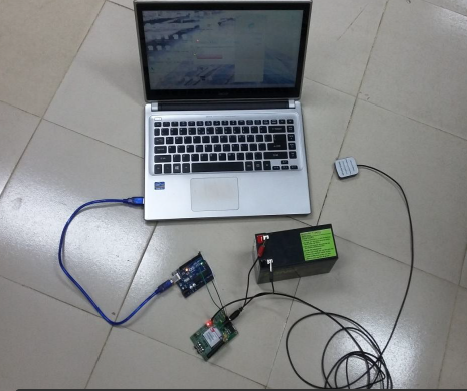
\includegraphics[width=.6\textwidth]{design-system}}
	\caption{سیستم ردیابی طراحی شده}
\end{figure}

\section{بررسی عملکرد سیستم ردیابی}
همانطور كه گفته شد، قسمت سخت‌ افزاری سیستم ما از چهار ماژول \lr{SIM808}، گیرنده \lr{GSM}، گیرنده \lr{GPS} و میکروکنترلر آردوینو تشکیل شده است. در اين قسمت، پياده‌سازي سيستم طراحی شده، شيوه ارتباط اجزای مختلف و كد پياده‌سازي شده را توضيح خواهیم داد.
\subsection{بررسی عملکرد مدار}
پيش از پرداختن به ماژول‌ها و شيوه اتصال آن‌ها، لازم است شيوه عملكرد ميكروكنترلر سيستم و نحوه پردازش اطلاعات را در فلوچارتي مشاهده كنيم. عملكرد كلي سيستم در بخش قبل توضيح داده شد. اكنون با ارئه فلوچارتي درباره الگوريتم پياده‌سازي شده می‌توانیم درك بهتري نسبت به روند كار در مدار سخت‌افزاری طراحی شده و كد نوشته شده براي آن داشته باشيم.

\newpage
فلوچارت شكل ۴-۲ روند كلي كد پياده‌سازي شده بر روي آردوینو را نمايش می‌دهد.
\begin{figure}[h!]
	\centering
	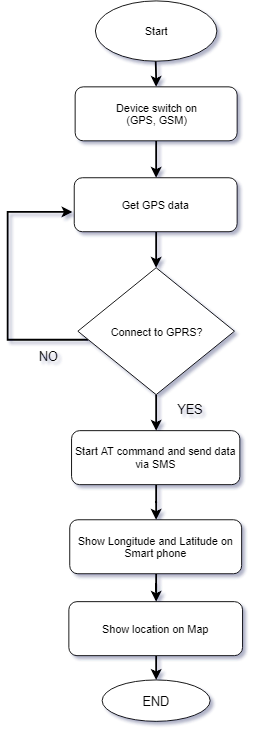
\includegraphics[width=.4\textwidth]{tracking-flowchart}
	\caption{عملکرد کد پیاده‌سازی شده بر روی آردوینو \cite{Rahman2016,Alshamsi,Hazza}}
\end{figure}



در ابتدای کار برای تست سیستم طراحی شده، آنتن \lr{GPS} به ماژول \lr{SIM808} متصل می‌شود تا موقعیت مکانی (طول و عرض جغرافیایی) شی را از ماهواره دریافت کند. برای انجام این کار از نرم‌افزار \lr{Arduino IDE} برای پروگرم کردن کد نوشته شده بر روی برد آردوینو استفاده می‌شود.\\
\\
در فلوچارت شکل ۴-۳ نحوه کار \lr{GPS} نشان داده شده است.
\begin{figure}[!h]
	\centerline{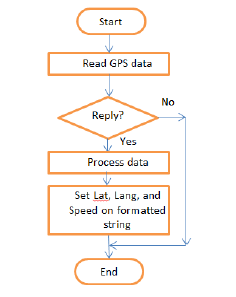
\includegraphics[width=.6\textwidth]{gps-flowchart}}
	\caption{فلوچارت خواندن اطلاعات \lr{GPS} \cite{ElShafee2013}}
\end{figure}
\\

برای ارسال موقعیت مکانی شی به کاربر از طریق شبکه \lr{GSM} از ماژول \lr{SIM808} و میکروکنترلر آردوینو متصل به آن استفاده می‌شود. برای ارتباط ماژول \lr{SIM808} با شبکه \lr{GSM} از دستورات \lr{AT} برای برنامه‌نویسی و کنترل آن استفاده می‌کنیم.\\

\newpage
در فلوچارت شکل ۴-۴ نحوه کار \lr{GSM} نشان داده شده است.\\
\begin{figure}[!h]
	\centerline{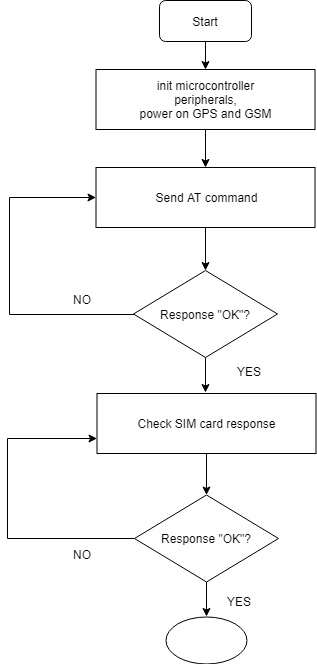
\includegraphics[width=.6\textwidth]{gsm-flowchart}}
	\caption{فلوچارت نحوه کار \lr{GSM} \cite{ElShafee2013}}
\end{figure}
\newpage
\begin{figure}[!h]
	\centerline{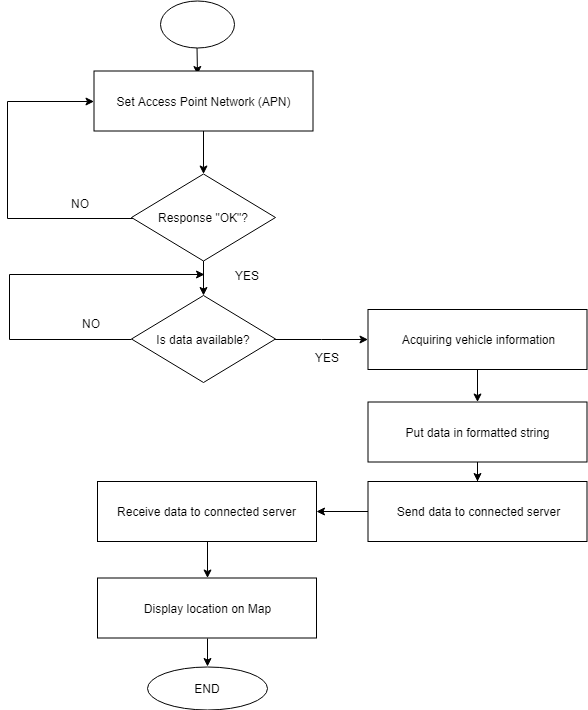
\includegraphics[width=.9\textwidth]{continue-gsm}}
	\caption{ادامه فلوچارت نحوه کار \lr{GSM} \cite{ElShafee2013}}
\end{figure}


سیستم ردیابی طراحی شده متشکل از ماژول \lr{SIM808} متصل به برد آردوینو می‌باشد. این ماژول دستور \lr{AT} را می‌فرستد، اگر جواب این دستور \lr{OK} باشد وضعیت شبکه چک می‌شود. بعد از چک شدن وضعیت شبکه و وصل شدن به آن، وضعیت \lr{GPS} چک شده و موقعیت مکانی شی از آن دریافت می‌شود. پس از دریافت اطلاعات جغرافیایی، درخواست ارسال اطلاعات به سرور ارسال می‌شود. در انتها داده ارسال شده در سمت سرور پردازش شده و مسیر حرکت شی بر روی نقشه نشان داده خواهد شد.
\\
\section{بررسی معماری مدار}
در این قسمت بخش سخت‌ افزاری سیستم پیشنهادی را توضیح می‌دهیم. همانطور که در قسمت‌های قبل مشخص شد، با استفاده از آنتن \lr{GPS} متصل به ماژول \lr{SIM808} اطلاعات مربوط به موقعیت مکانی، از هر دو دقیقه یکبار از ماهواره دریافت شده و سپس از طریق شبکه \lr{GSM} به سرور فرستاده می‌شود. \\
در شکل ۴-۷ شیوه اتصال ماژول \lr{SIM808} به آردوینو را مشاهده می‌کنید.\\

\begin{figure}[!h]
	\centerline{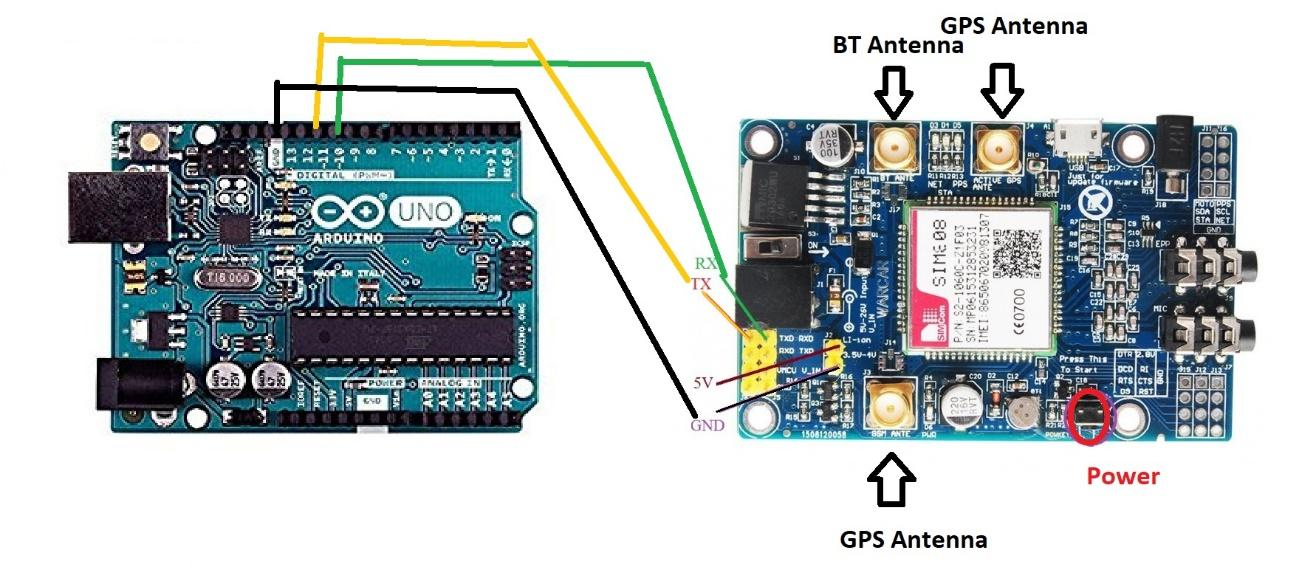
\includegraphics[width=.8\textwidth]{sim808-arduino}}
	\caption{شیوه اتصال آردوینو به ماژول \lr{SIM808} \cite{interface}}
\end{figure}


ماژول \lr{SIM808} با استفاده از رابط سریال به آردوینو متصل شده است، دارای دو پایه \lr{TX} و \lr{RX} است که به ترتیب به پایه دیجیتال ۱۰ و ۱۱ آردوینو متصل شده‌اند. پایه اتصال به زمین این ماژول هم به پایه اتصال به زمین برد آردوینو متصل شده است. ولتاژ موردنیاز ماژول \lr{SIM808} را از طریق آداپتور ۹ ولت خروجی تامین می‌کنیم. 
\newpage
\section{برنامه کاربردی}
شکل زیر معماری پیاده‌سازی شده در سیستم ردیابی پیشنهادی را نشان می‌دهد:

\begin{figure}[!h]
	\centerline{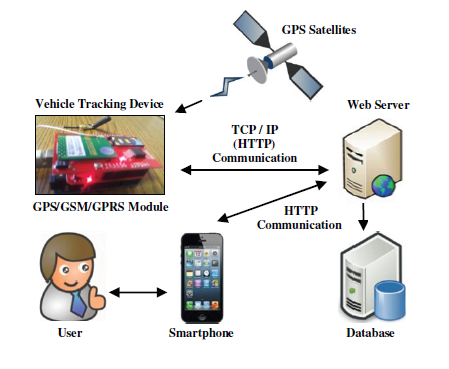
\includegraphics[width=.7\textwidth]{softarc}}
	\caption{معماری سیستم طراحی شده \cite{one}}
\end{figure}

در قسمت بک‌اند یک وب سرویس با معماری \lr{RESTful} توسعه داده شده است که این وب سرویس داده‌های دریافتی را در پایگاه داده موردنظر ذخیره می‌کند و برنامه تحت وب این اطلاعات را دریافت کرده و نمایش می‌دهد.


 \lr{REST}
یک معماری وب سرویس است که از \lr{HTTP} برای تبادل اطلاعات میان دو سیستم استفاده می‌کند. ایده اصلی این معماری این است که به جای استفاده از مکانیزم‌های پیچیده برای اتصال ماشین‌ها از \lr{HTTP} برای برقراری اطلاعات بین ماشین‌ها استفاده کند.\\
در این قسمت ابتدا ساختار پایگاه داده و شیوه ارتباط با آن را بیان می‌کنیم. در پایان نیز برنامه تحت وب نوشته شده را که مسیر حرکت شی را بر روی نقشه نمایش می‌دهد، را توضیح می‌دهیم.
\subsection{پایگاه داده}
برای ذخیره اطلاعات و مدیریت سرور از از پایگاه داده مانگو\RTLfootnote{\lr{MongoDB}} استفاده کرده‌ایم. مانگو دی‌بی یک پایگاه داده \lr{NOSQL} است که روی سیستم عامل‌های مختلف از جمله ویندوز، مکینتاش و لینوکس اجرا می‌شود و همچنین اغلب زبان‌های برنامه‌نویسی را پشتیبانی می‌کند. مانگو دی‌بی کارایی بالا، دسترس پذیری، مقیاس پذیری، قابلیت تکرارهای سریع واشتراک پذیری خودکار را فراهم می‌کند. مانگو دی‌بی به دلیل ساختار \lr{NOSQL} تنها داده‌ها را ذخیره و جستجو می‌کند و در نتیجه سرعت دستیابی و ذخیره داده‌ها به شدت افزایش می‌یابد.
\\
در پایگاه داده اطلاعات دریافتی از سمت سخت‌افزار، که هر دو دقیقه یکبار موقعیت شی از ماهواره دریافت می‌شود، را ذخیره می‌کنیم که این اطلاعات شامل طول و عرض جغرافیایی، سرعت، زمان و تاریخ است.
\subsection{نمایش اطلاعات}
\subsubsection{وب اپلیکیشن}
برای نمایش اطلاعات دخیره شده در پایگاه داده، یک وب اپلیکیشن توسعه داده شده است. قسمت فرانت‌اند این وب ابلیکیشن با استفاده از فریم‌ورک \lr{Angular} پیاده‌سازی شده و برای نمایش مسیر حرکت شی از \lr{Google Map} استفاده می‌کنیم. \\این وب اپلیکیشن از طریق آدرس زیر در دسترس است: \href{http://103.216.62.79}{\lr{http://103.216.62.79}}


پردازش‌های سمت سرور با استفاده از فریم‌ورک \lr{Express} پیاده‌سازی شدند. نحوه عملکرد کد سمت سرور به این صورت است که به محض دریافت داده‌های جدید از سمت سخت‌افزار، این داده‌ها در پایگاه داده مانگو ذخیره می‌شوند. سخت‌افزار برای فرستادن داده جدید به سرور، هر بار یک درخواست \lr{HTTP} به این شکل به سرور می‌فرستد: \lr{/api/device/add/}


کد نوشته شده در سمت سرور به این صورت عمل می‌کند که هر ۶۰ ثانیه یکبار به پایگاه داده مراجعه می‌کند و با توجه به آخرین زمان دریافت اطلاعات از آن، اطلاعات دریافتی از  آن زمان به بعد را دریافت کرده و بدین ترتیب مسیر حرکت شی را بر روی نقشه نمایش می‌دهد.
\newpage
شکل ۴-۷ برنامه کاربردی طراحی شده را نمایش می‌دهد.
\\
 \begin{figure}[!h]
 	\centerline{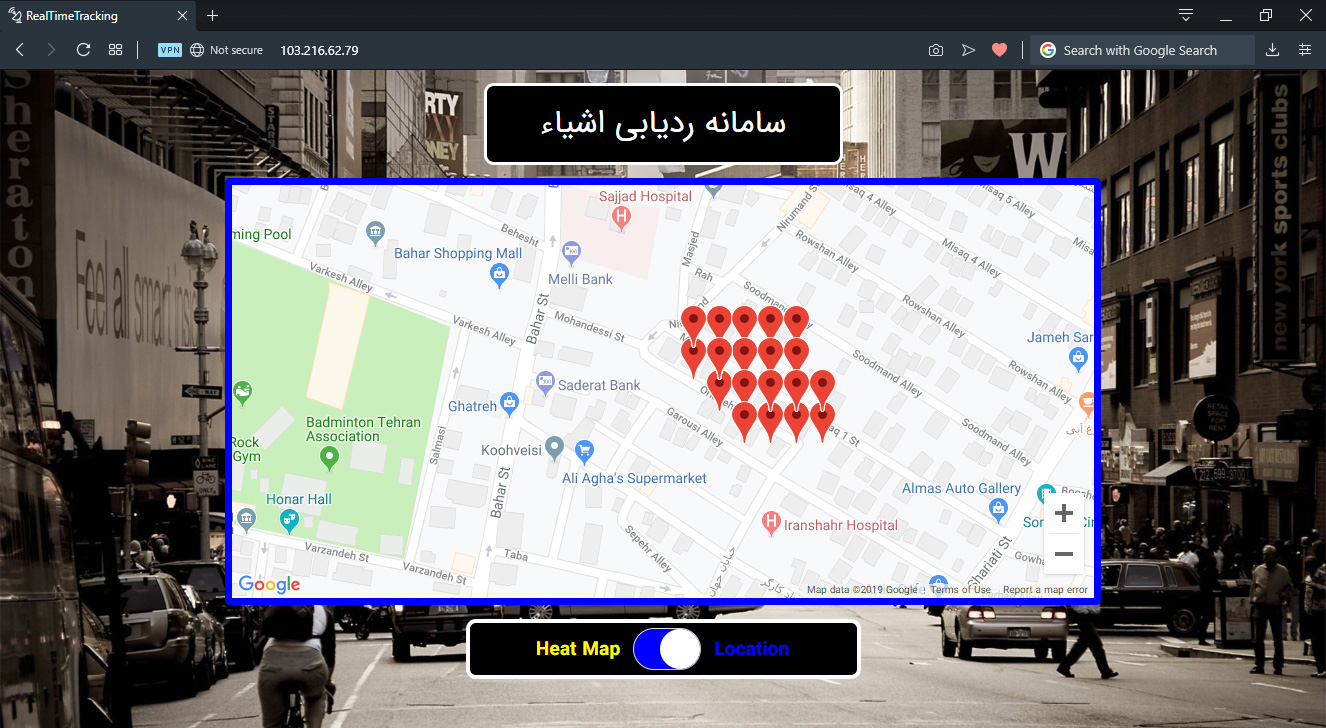
\includegraphics[width=.9\textwidth]{webapp3}}
 	\caption{نمایش مسیر جرکت شی در برنامه کاربردی}
 \end{figure}
\\
 اگر بر روی هر کدام از مارکرهای موجود در نقشه که بیانگر موقعیت شی در هر لحظه می‌باشند، کلیک کنیم میتوان سرعت حرکت شی، زمان و تاریخ را در آن موقعیت را مشاهده خواهیم کرد. در شکل زیر نمایی از این خروجی را مشاهده می‌کنیم:
  \begin{figure}[!h]
 	\centerline{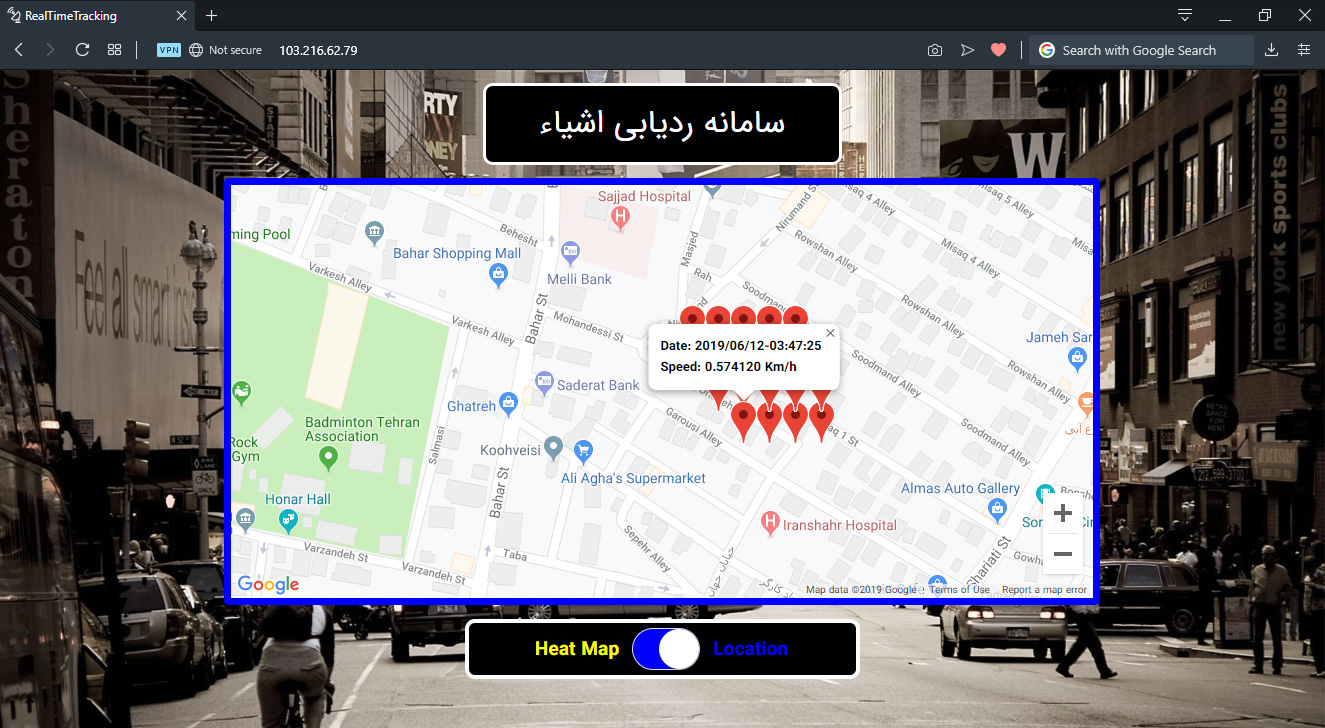
\includegraphics[width=.9\textwidth]{webapp4}}
 	\caption{نمایش سرعت، زمان و تاریخ حرکت شی در هر موقعیت بر روی نقشه}
 \end{figure}
 \subsubsection{پیام کوتاه}
 یکی از قابلیت‌های منحصر به فرد سیستم ردیابی پیاده‌سازی شده این است که میتوان به شماره سیم‌کارت درج شده بر روی ماژول \lr{SIM808}، برای دریافت موقعیت فعلی شی موردنظر، پیامی فرستاد. این ماژول هم پس از دریافت پیام، موقعیت مکانی شی را از طریق \lr{GPS} دریافت کرده و اطلاعات لازم برای ردیابی را در پاسخ به پیام دریافتی ارسال می‌کند. این اطلاعات شامل طول و عرض جغرافیایی و سرعت شی می‌باشد. همچنین یک لینک هم به این پیام پیوست شده است که کاربر با کلیک بر روی آن می‌تواند موقعیت شی را بر روی نقشه مشاهده نماید.\\
در شکل‌های زیر پیام ارسال شده و پاسخ آن از طریق سیستم طراحی شده را مشاهده می‌کنید.\\
 \begin{figure}[!h]
	\centerline{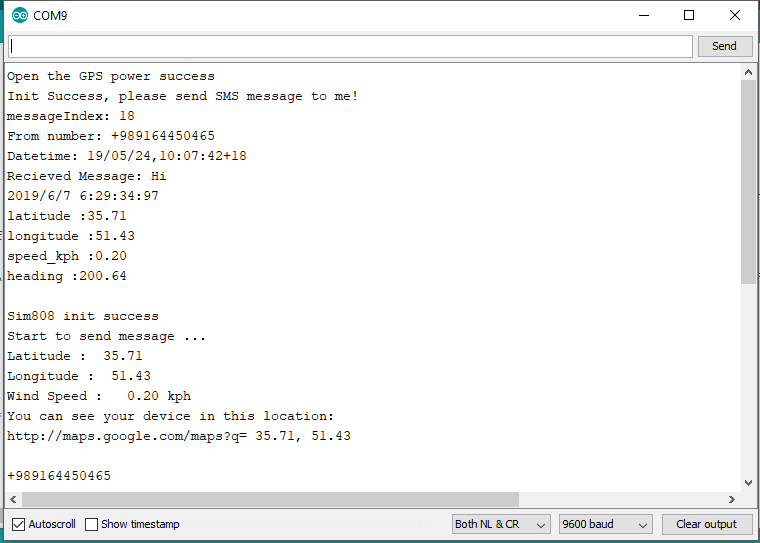
\includegraphics[width=.9\textwidth]{msg}}
	\caption{دریافت پیام ارسالی کاربر برای دریافت موقعیت توسط ماژول \lr{SIM808}}
\end{figure}
\newpage
شکل ۴-۱۰ پیام ارسال شده برای کاربر را نشان می‌دهد.
 \begin{figure}[!h]
 	\centerline{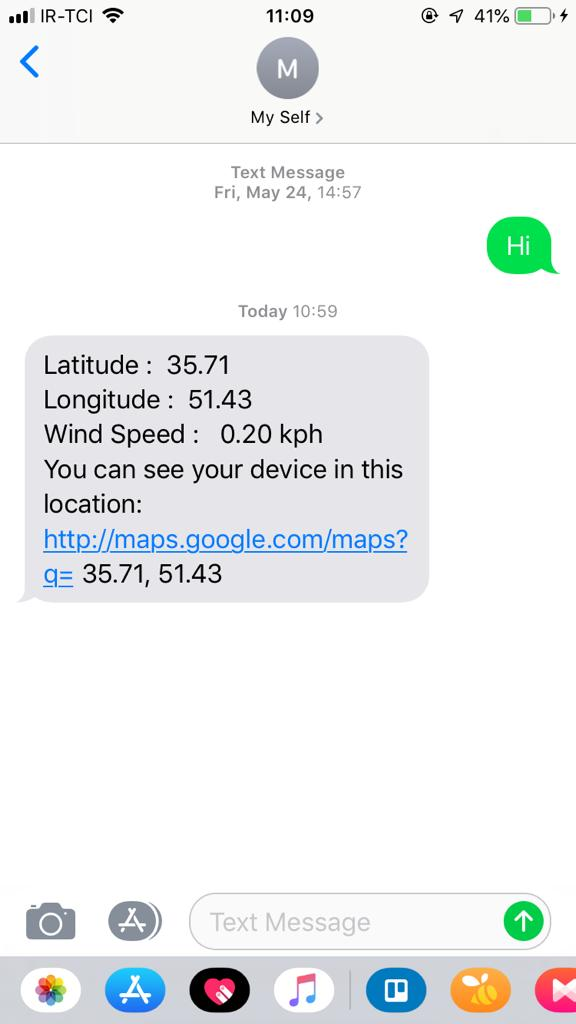
\includegraphics[width=.3\textwidth]{sms}}
 	\caption{پیام دریافت شده توسط کاربر}
 \end{figure}
\\
با کلیک بر لینک دریافت شده میتوان موقعیت فعلی شی را بر روی نقشه مشاهده نمود.\\
 \begin{figure}[!h]
	\centerline{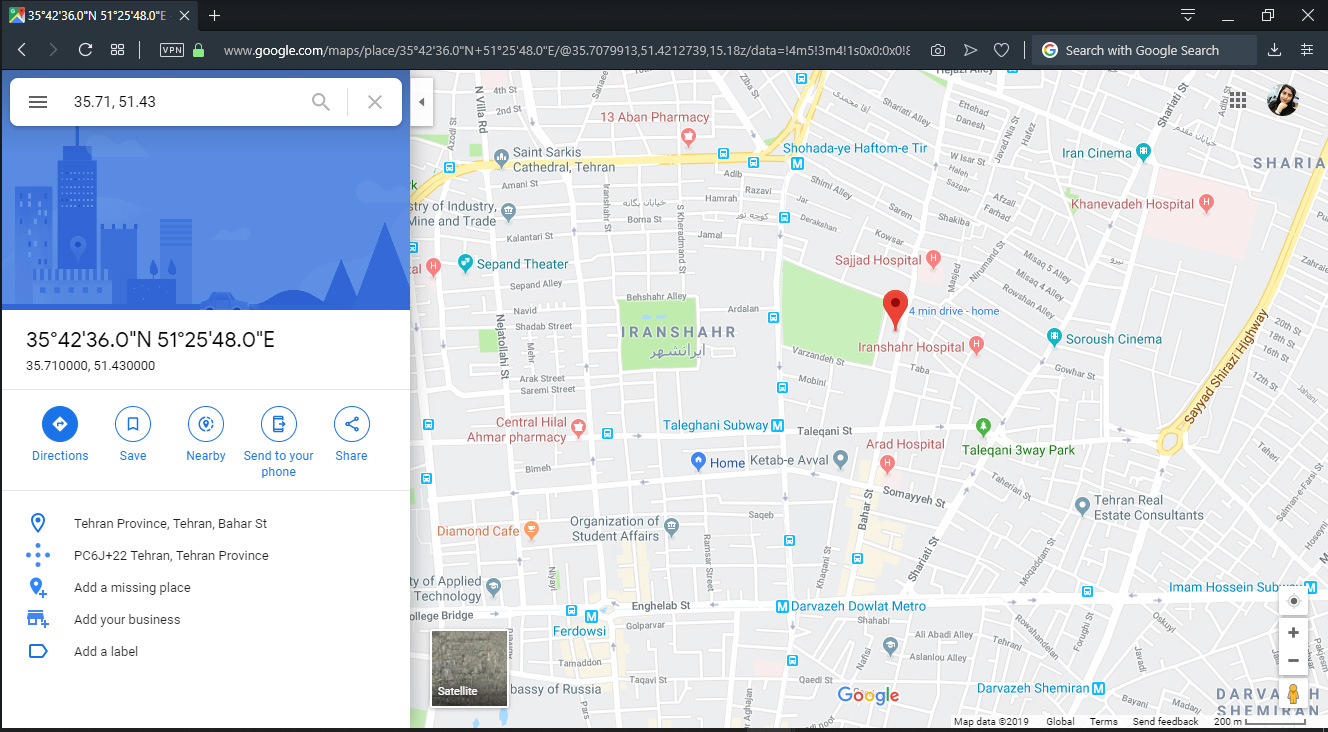
\includegraphics[width=.8\textwidth]{map}}
	\caption{مشاهده موقعیت شی بر روی نقشه}
\end{figure}
\newpage
\section{تحلیل اطلاعات} 
با استفاده از سیستم ردیابی بی‌درنگ طراحی شده، توانستیم موقعیت مکانی شی رو به طور پیوسته اندازه‌گیری کرده و این اطلاعات را در پایگاه داده ذخیره کنیم.
یکی دیگر از قابلیت‌های این سیستم بدست آوردن مکان‌های پر تردد فرد در یک بازه زمانی مشخص است. برای این کار از هیت مپ (نقشه حرارتی)\RTLfootnote{\lr{Heat Map}} استفاده کردیم.


هیت مپ داده‌های گرافیکی و رنگی هستند که ما را قادر می‌سازند تا رفتار کاربرانمان را شناسایی کنیم. در این پروژه، هیت مپ را با استفاده از اطلاعات ذخیره شده که در واقع موقعیت‌های مکانی شی دز زمان‌های مختلف بوده است، پیاده سازی کردیم. مکان‌های پرتردد فرد که فراوانی آن‌ها در مجموعه داده ما بیشتر از بقیه بوده، به صورت نواحی قرمز رنگ بر روی نقشه قابل مشاهده خواهند بود.


برنامه کاربردی طراحی شده شامل دو نقشه است. به این صورت است که در ابتدا موقعیت‌های شی را بر روی نقشه نشان می‌دهد و با انتخاب گزینه هیت‌مپ میتوان هیت مپ این نقاط را مشاهده نمود. در شکل ۴-۱۰ بر روی هیت مپ مکان‌های پرتردد شی که به صورت نواحی قرمزرنگ نشان داده است را مشاهده می‌کنید.

 \begin{figure}[!h]
	\centerline{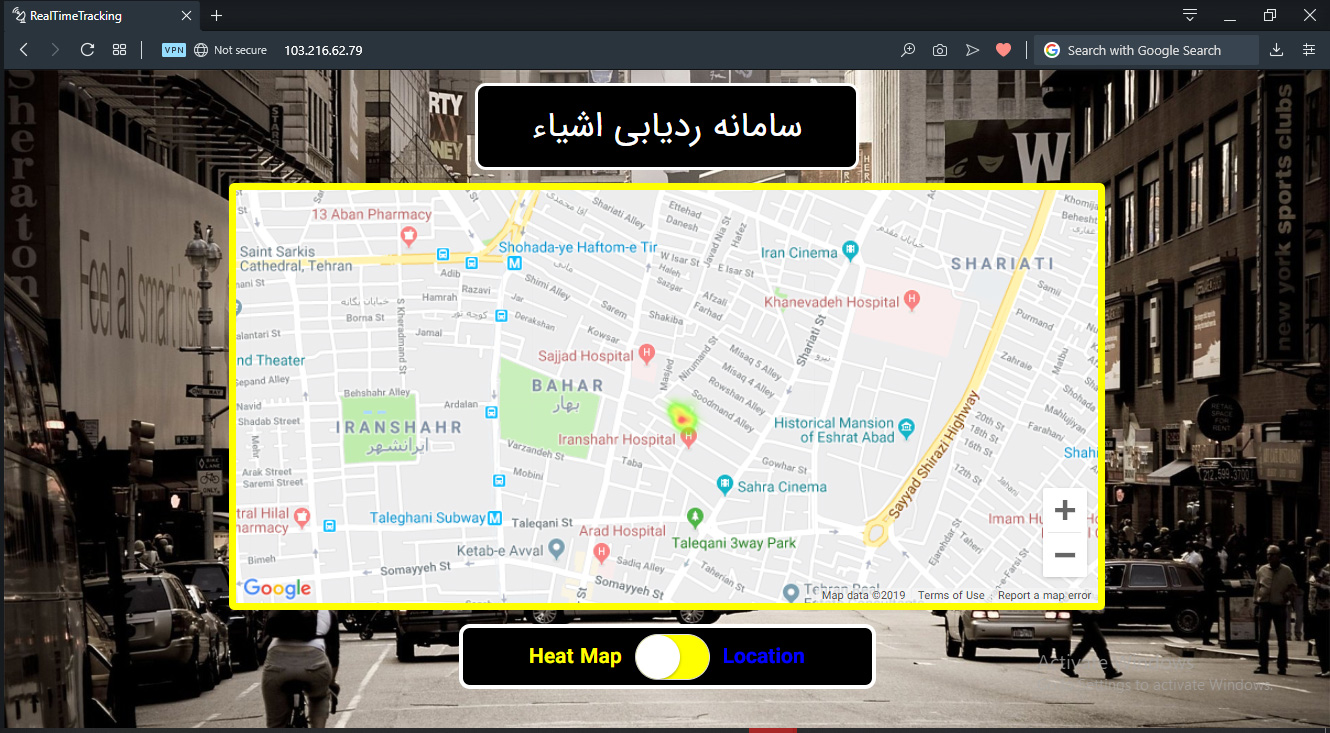
\includegraphics[width=.9\textwidth]{heatmap2}}
	\caption{مکان‌های پرتردد شی بر روی هیت مپ}
\end{figure}


\chapter{جمع‌بندي و کارهای آتی}
\section{جمع‌بندی}
در این پروژه هدف ما پیاده‌سازی یک سیستم ردیابی بی‌درنگ برای ردیابی اشیا متحرک بوده است.  لذا در این پروژه سیستم ردیابی، برای مانیتور کردن موقعیت شی متحرک از طریق پیام کوتاه و همچنین به صورت آنلاین بر روی نقشه تست و پیاده‌سازی نمودیم. هسته اصلی سیستم طراحی شده، برد آردوینو و ماژول سیم ۸۰۸ می‌باشد. مودم جی‌اس‌ام با استفاده از دستورات \lr{AT} کنترل شده و از این طریق امکان تبادل اطلاعات با استفاده از شبکه جی‌اس‌ام را فراهم می‌آورد. در این پروژه برای یافتن موقعیت شی از ماژول جی‌پی‌اس استفاده شده است. جی‌پی‌اس هر دو دقیقه یکبار موقعیت مکانی شی را از ماهواره دریافت کرده و این اطلاعات به سمت سرور فرستاده می‌شوند. سرور اطلاعات دریافتی را برای وب سرویس پیاده‌سازی شده، ارسال می‌کند. در نهایت این داده‌ها در پایگاه داده ذخیره شده و در برنامه کاربردی نمایش داده می‌شوند و میتوانیم مسیر حرکت شی را بر روی نقشه مشاهده کنیم.


برنامه پیاده‌سازی شده بر روی آردوینو به این صورت نوشته شده است که هر دو دقیقه یکبار موقعیت مکانی شی را با استفاده از جی‌پی‌اس دریافت می‌کند و به سرور می‌فرستد. در سمت سرور  این اطلاعات در پایگاه داده مانگو ذخیره شده و سپس با استفاده از این اطلاعات مسیر حرکت شی بر روی نقشه داده می‌شود. کد سمت سرور به این صورت نوشته شده است که هر یک دقیقه یکبار به پایگاه داده مراجعه کرده و نقشه حاوی مسیر حرکت شی به‌روزرسانی می‌شود.


در پایان این پروژه توانستیم سیستم ردیابی بی‌درنگی را  طراحی کنیم که امروزه دارای کاربرد فراوان در زمینه‌های مختلف مانند ردیابی وسایل نقلیه، کودکان و سالمندان و ... می‌باشد و با استفاده از آن قادر خواهیم بود اقدامات لازم را در سریع‌ترین زمان ممکن انجام دهیم.

%--------------------------------------------------------------------------appendix( مراجع و پیوست ها)
\chapterfont{\vspace*{-2em}\centering\LARGE}%

\appendix
\bibliographystyle{plain-fa}
\bibliography{references}
\chapter*{‌پیوست}
\begin{enumerate}
	\item \textbf{کد پیاده‌سازی شده بر روی آردوینو}
	\\
	\begin{figure}[!h]
		\centerline{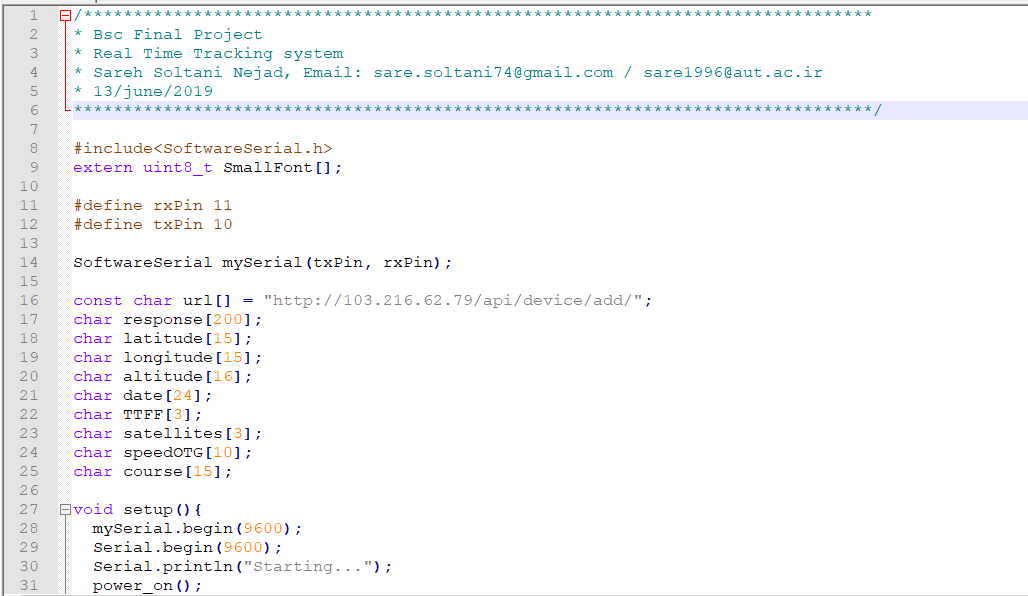
\includegraphics[width=1.1\textwidth]{code1}}
	\end{figure}
\newpage
	\begin{figure}[!h]
		\centerline{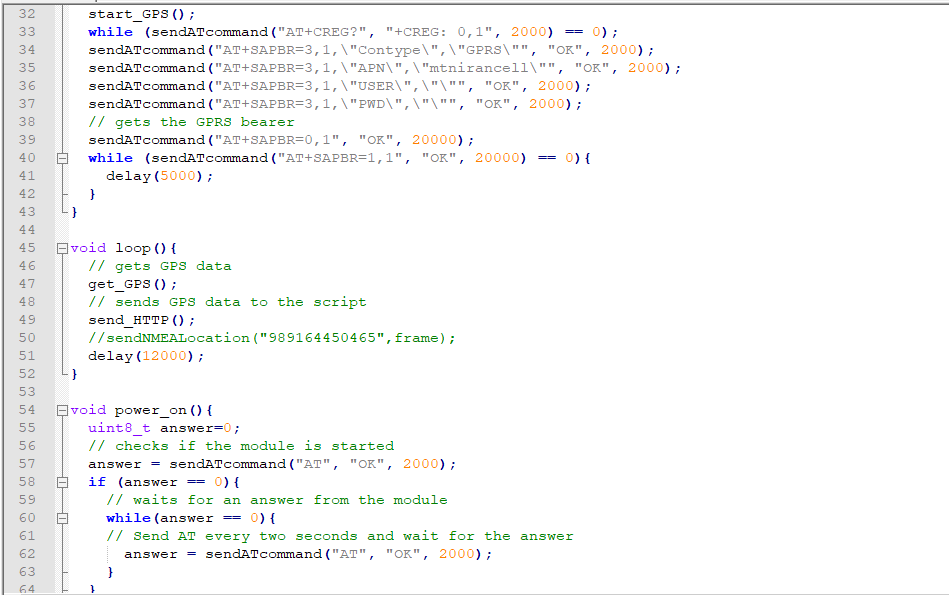
\includegraphics[width=1.1\textwidth]{code2}}
	\end{figure}
	\begin{figure}[!h]
		\centerline{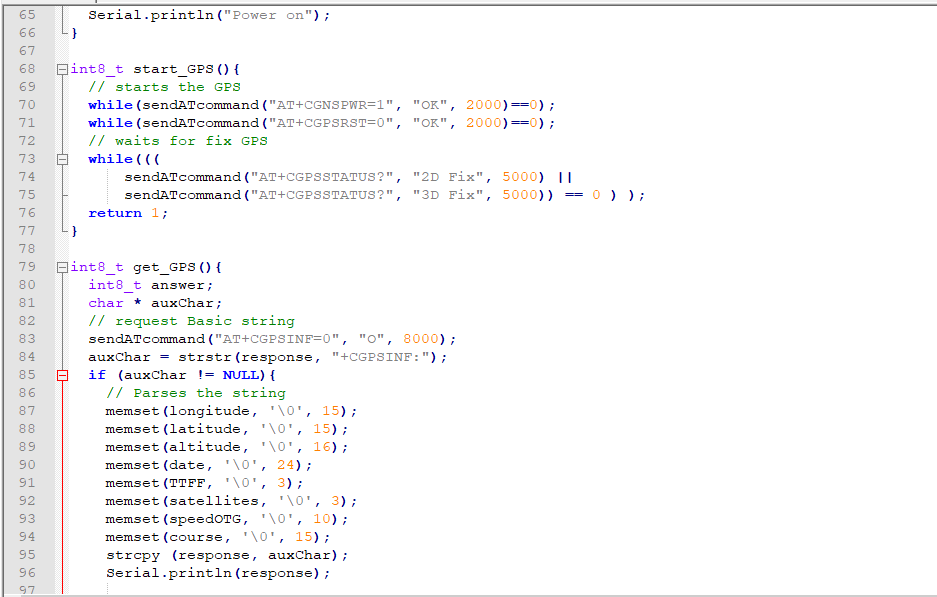
\includegraphics[width=1.1\textwidth]{code3}}
	\end{figure}
\newpage
	\begin{figure}[!h]
		\centerline{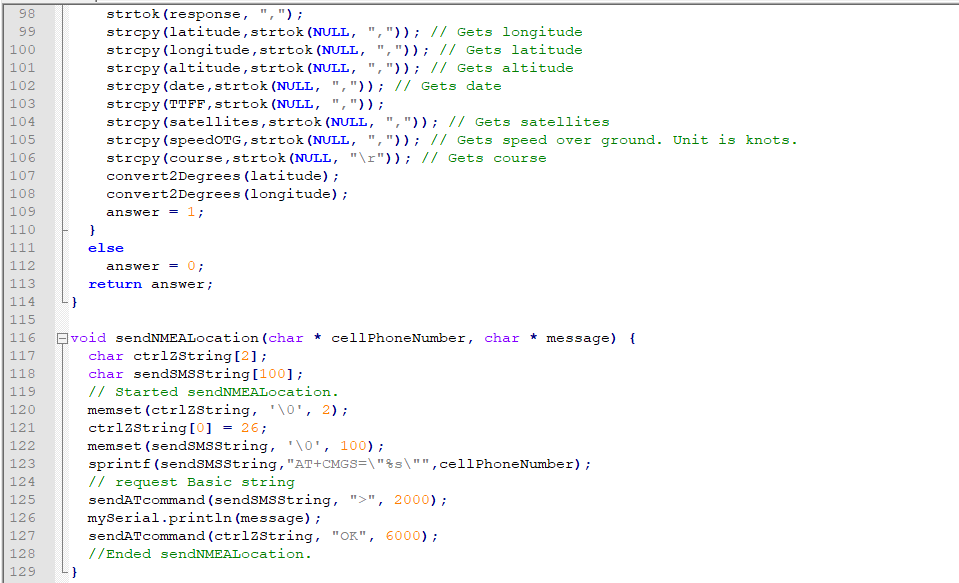
\includegraphics[width=1.1\textwidth]{code4}}
	\end{figure}
	\begin{figure}[!h]
		\centerline{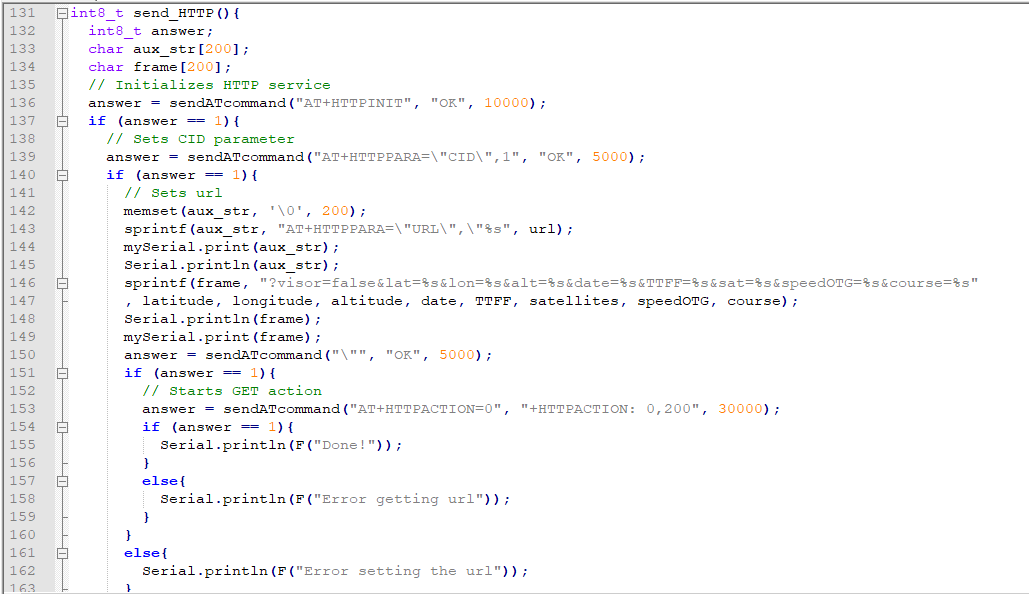
\includegraphics[width=1.1\textwidth]{code5}}
	\end{figure}
\newpage
	\begin{figure}[!h]
		\centerline{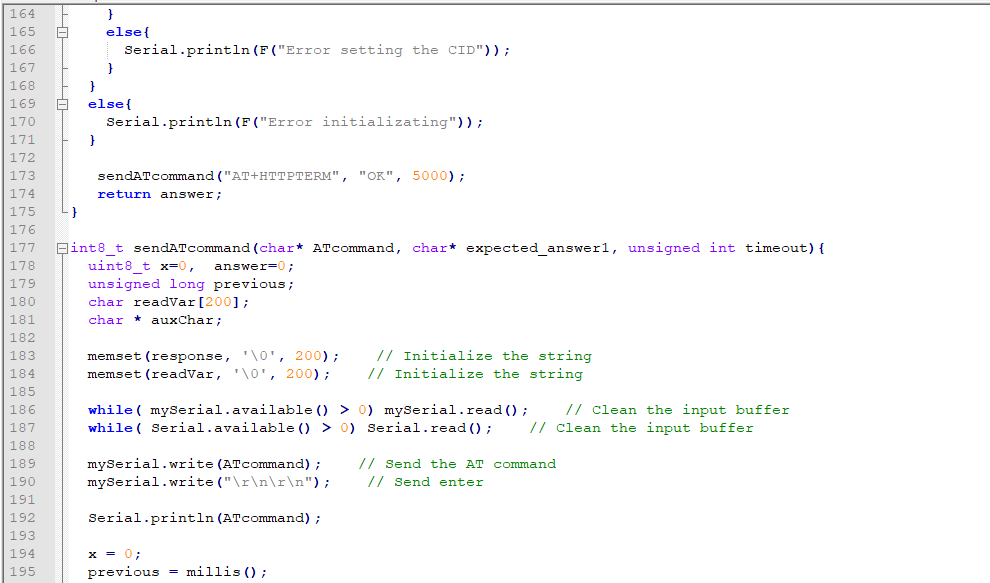
\includegraphics[width=1.1\textwidth]{code6}}
	\end{figure}
	\begin{figure}[!h]
		\centerline{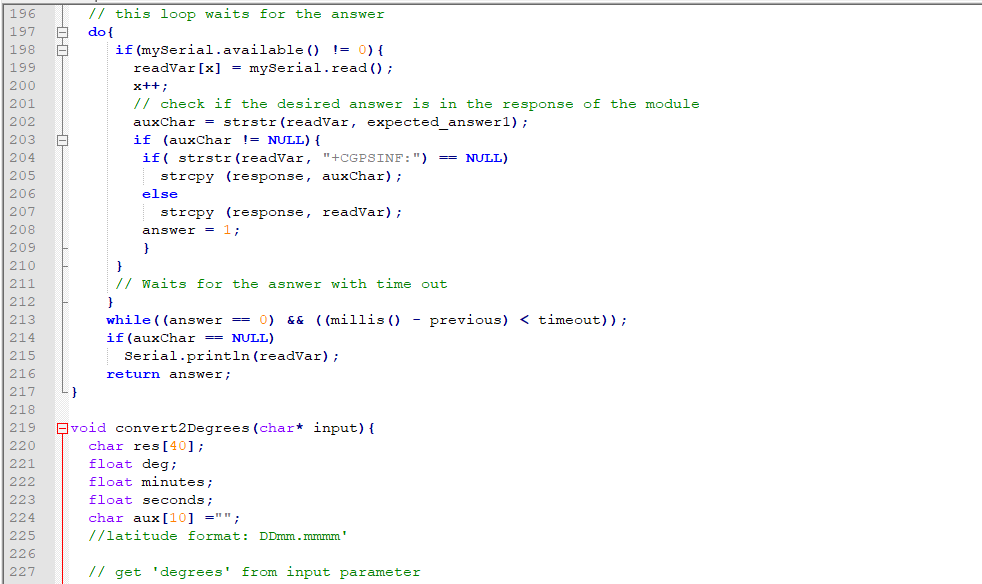
\includegraphics[width=1.1\textwidth]{code7}}
	\end{figure}
\newpage
	\begin{figure}[!h]
		\centerline{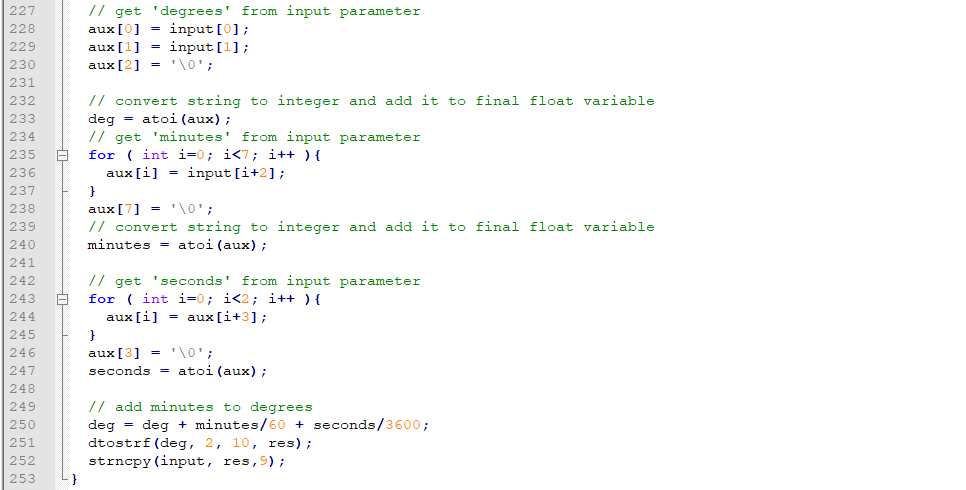
\includegraphics[width=1.1\textwidth]{code8}}
	\end{figure}
	\item \textbf{کد پیاده‌سازی شده سمت بک‌اند}
	\\
	\begin{figure}[!h]
		\centerline{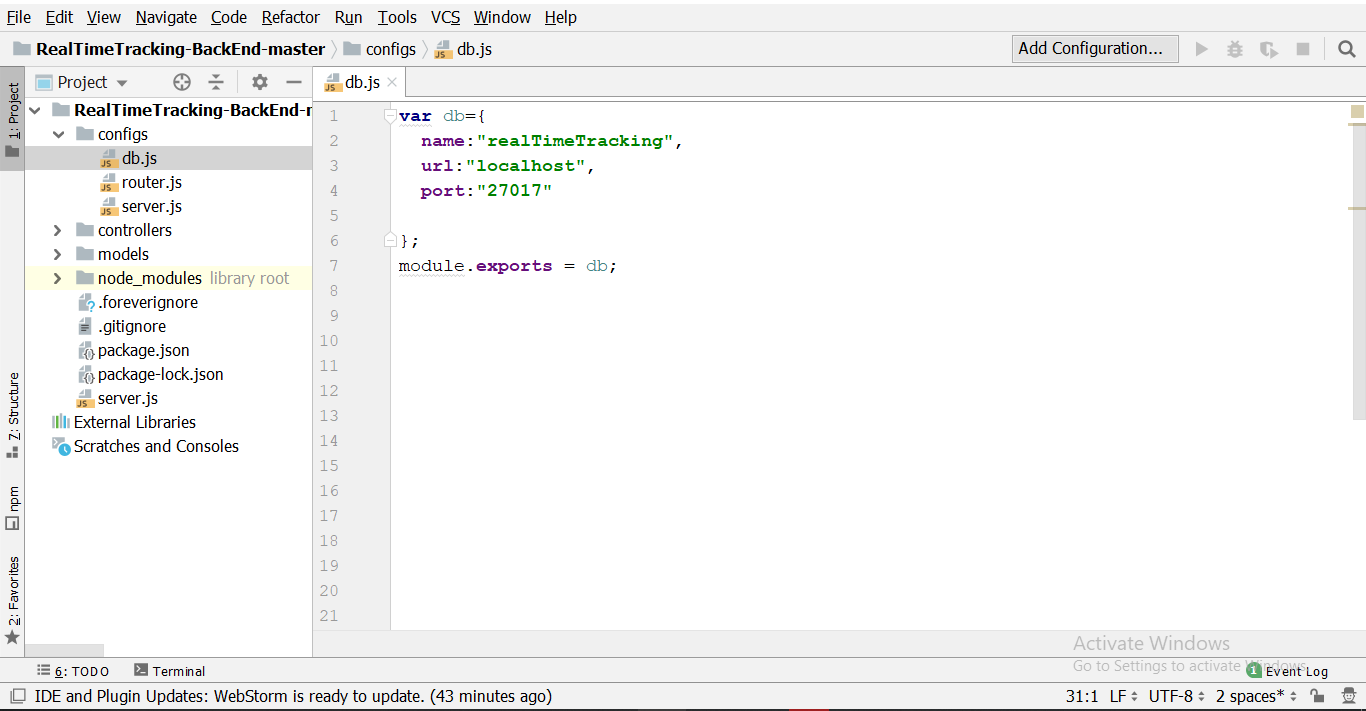
\includegraphics[width=1.1\textwidth]{code9}}
	\end{figure}
\newpage
	\begin{figure}[!h]
		\centerline{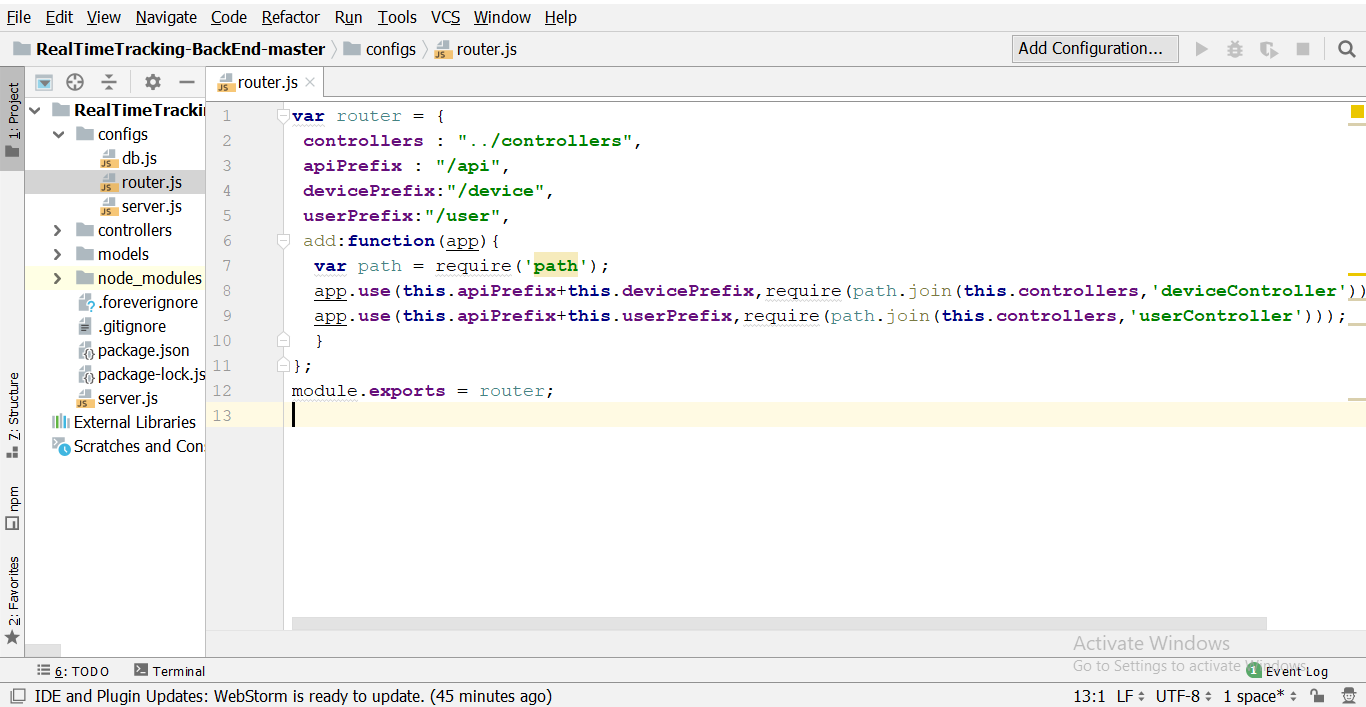
\includegraphics[width=1.1\textwidth]{code10}}
	\end{figure}
	\begin{figure}[!h]
		\centerline{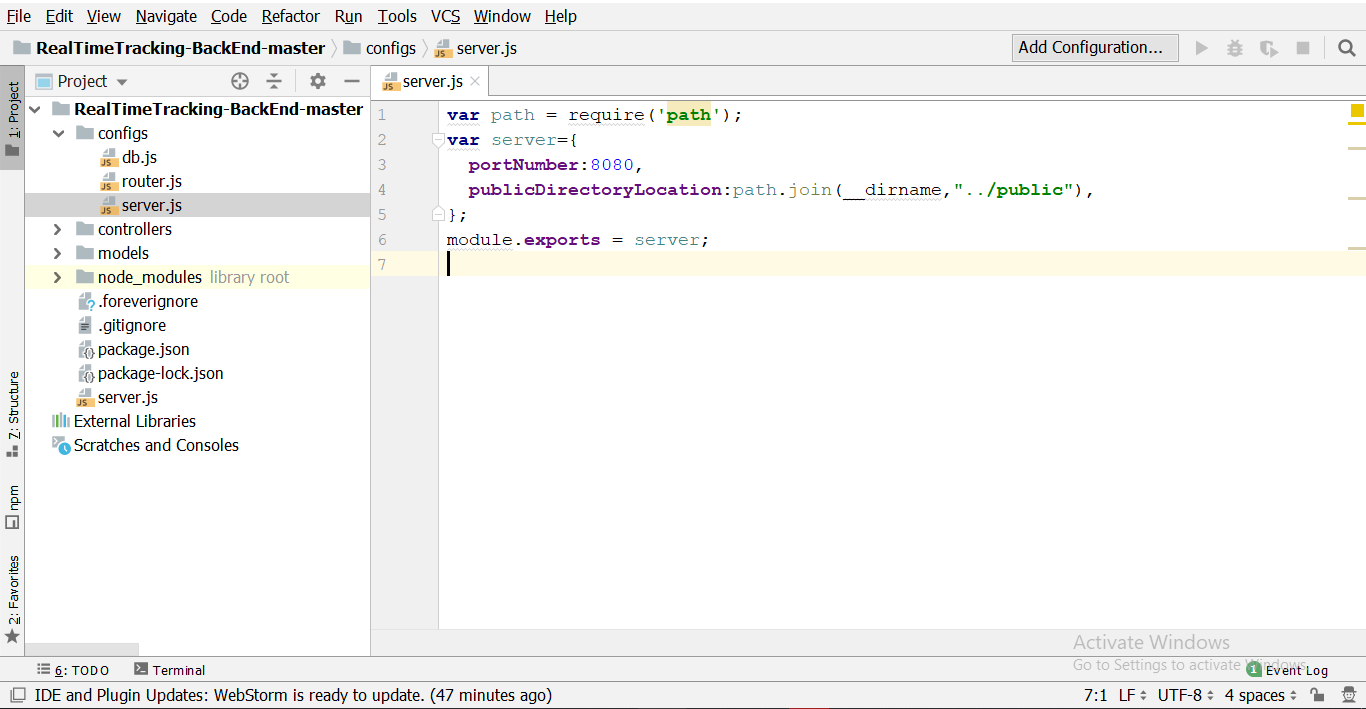
\includegraphics[width=1.1\textwidth]{code11}}
	\end{figure}
\newpage
	\begin{figure}[!h]
		\centerline{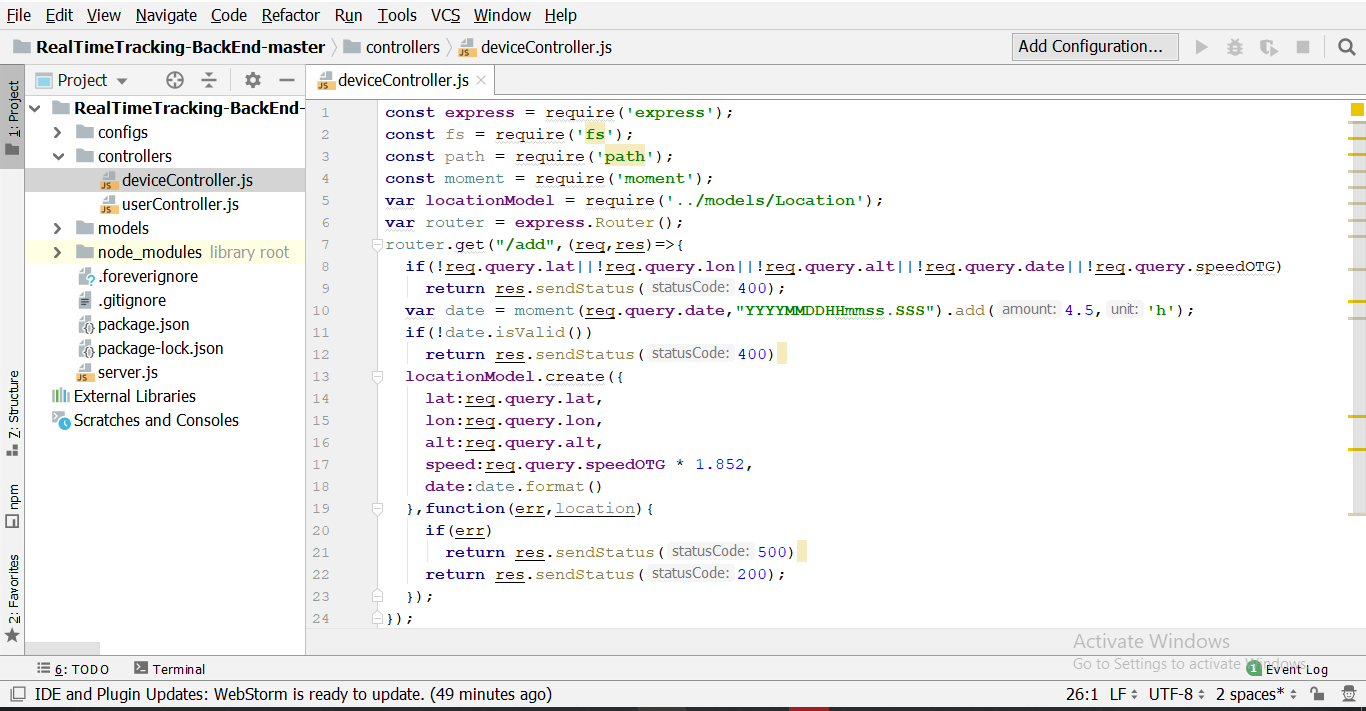
\includegraphics[width=1.1\textwidth]{code12}}
	\end{figure}
	\begin{figure}[!h]
		\centerline{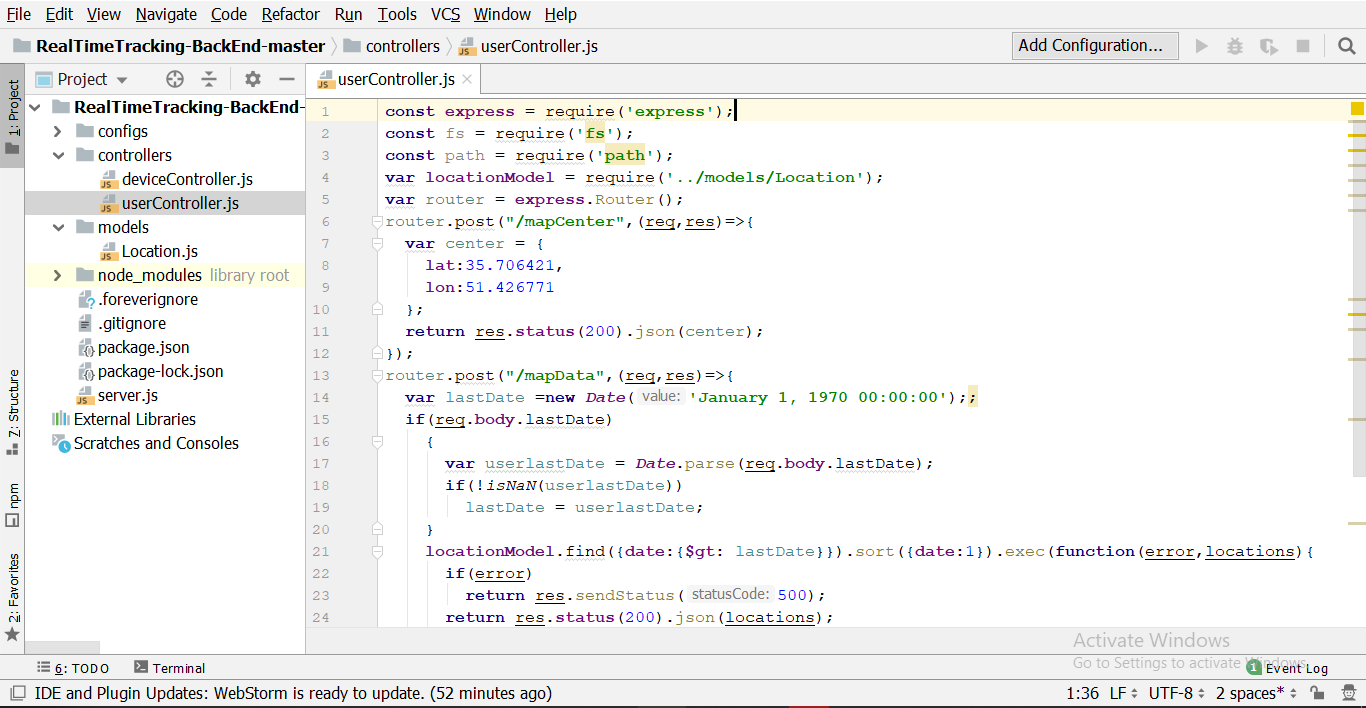
\includegraphics[width=1.1\textwidth]{code13}}
	\end{figure}
\newpage
	\begin{figure}[!h]
		\centerline{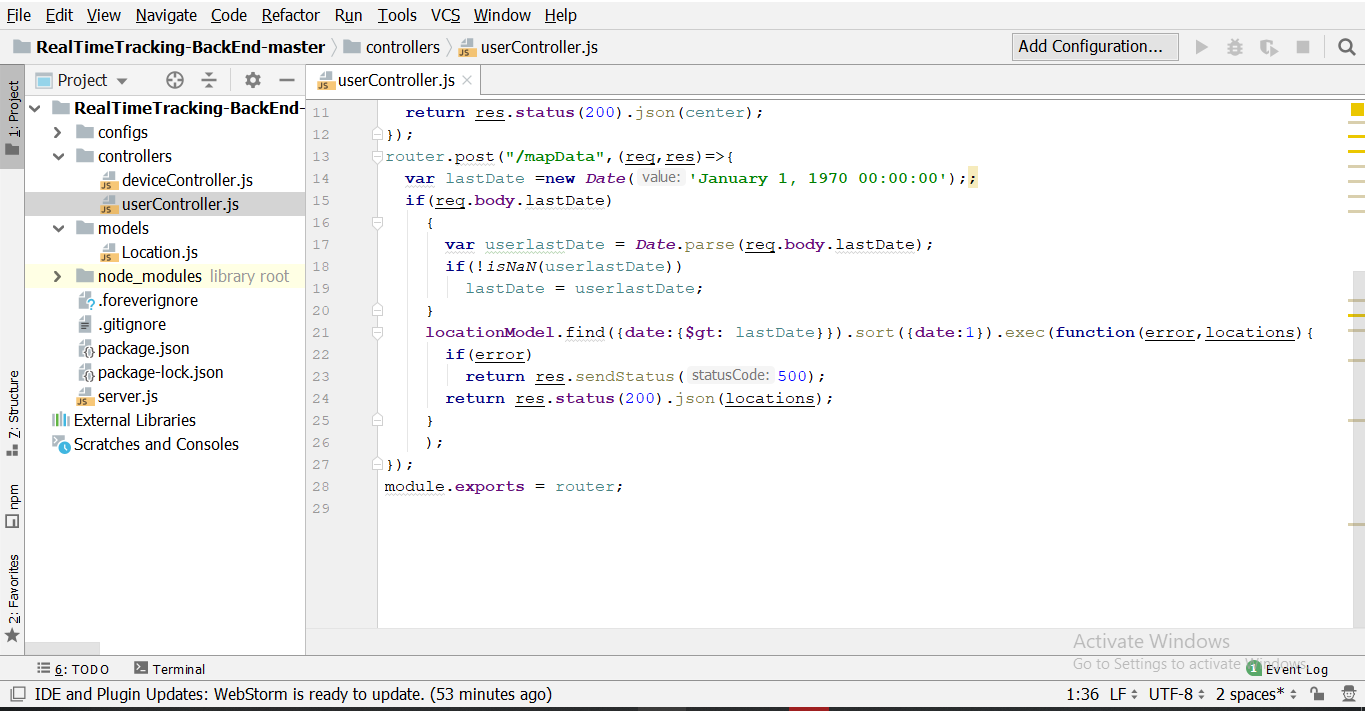
\includegraphics[width=1.1\textwidth]{code14}}
	\end{figure}
	\begin{figure}[!h]
		\centerline{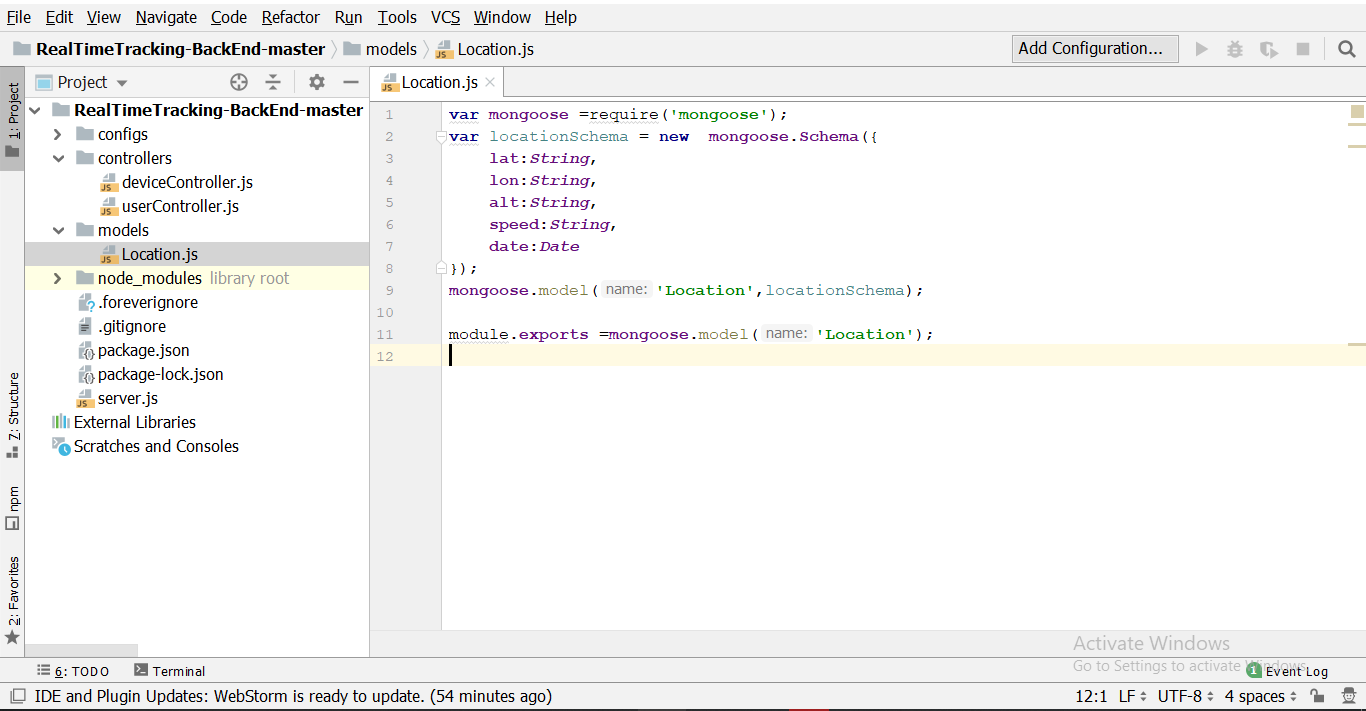
\includegraphics[width=1.1\textwidth]{code15}}
	\end{figure}
\newpage
	\item \textbf{کد پیاده‌سازی شده سمت فرانت‌اند}
	\\
	\begin{figure}[!h]
		\centerline{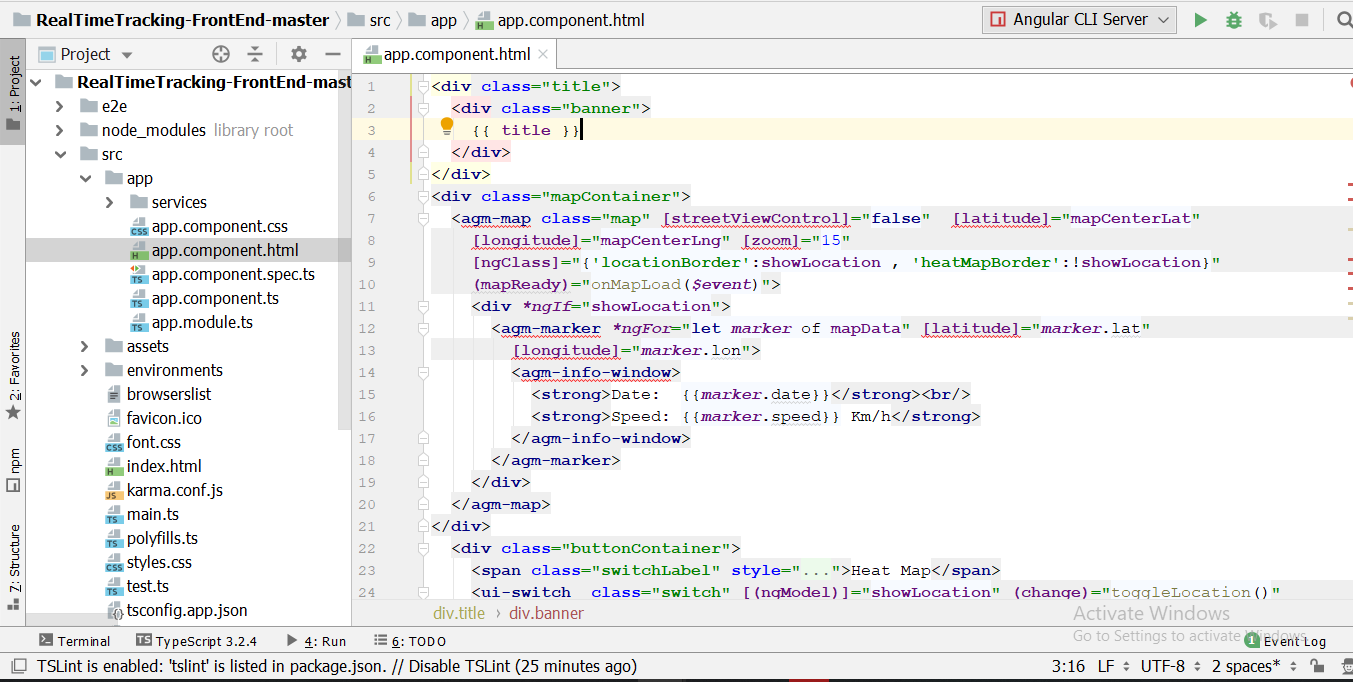
\includegraphics[width=1.1\textwidth]{code16}}
	\end{figure}
	\begin{figure}[!h]
		\centerline{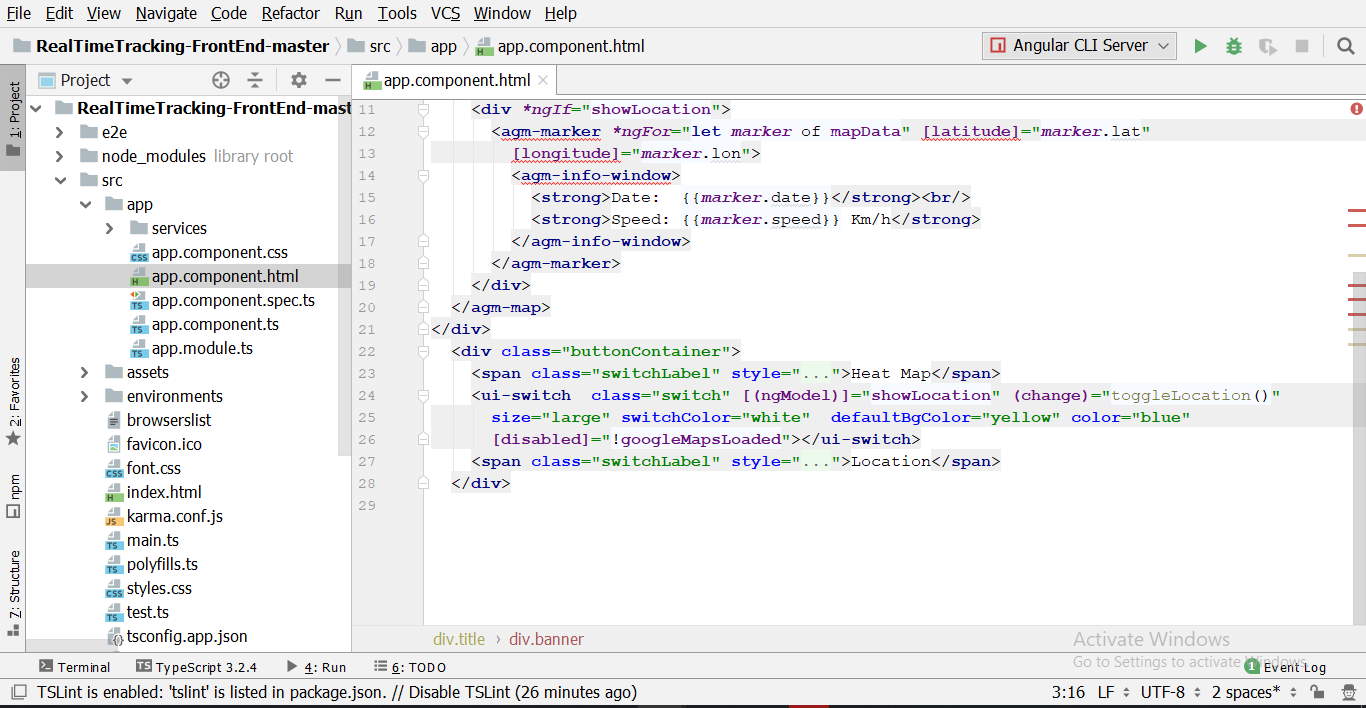
\includegraphics[width=1.1\textwidth]{code17}}
	\end{figure}
	\begin{figure}[!h]
		\centerline{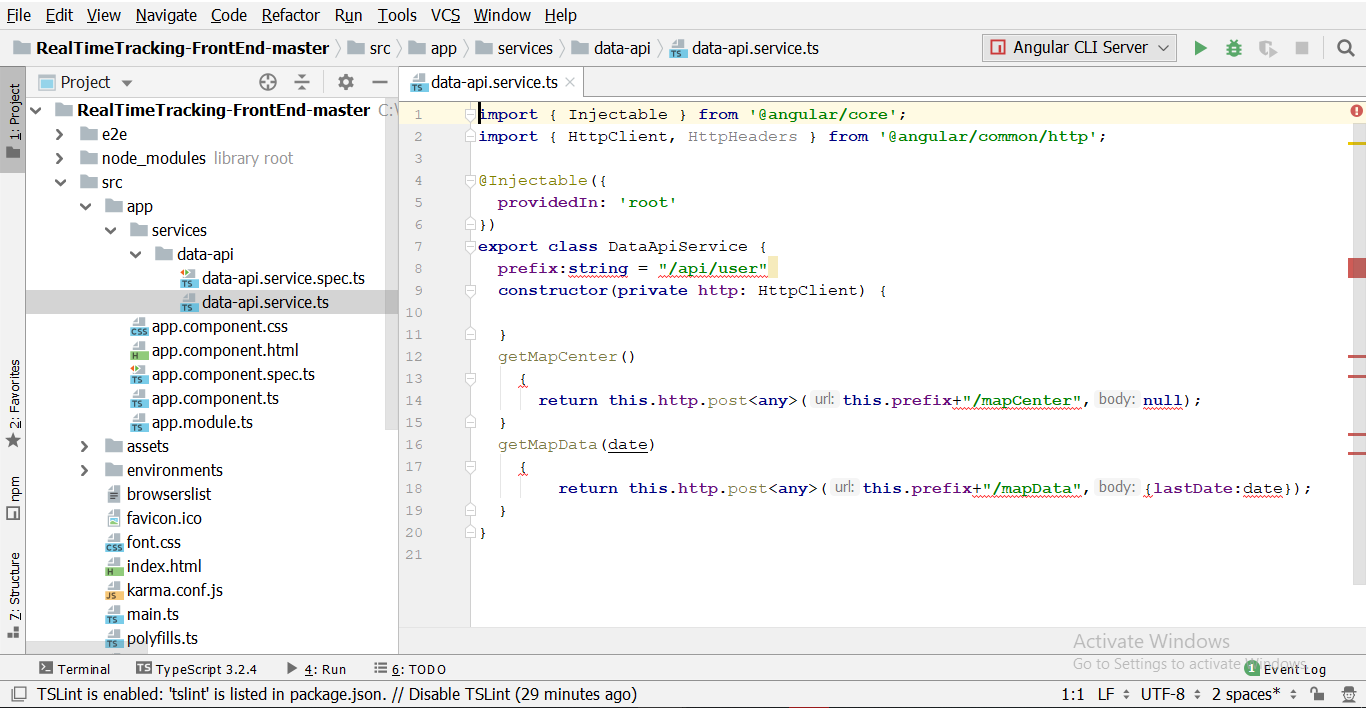
\includegraphics[width=1.1\textwidth]{code18}}
	\end{figure}
	\begin{figure}[!h]
		\centerline{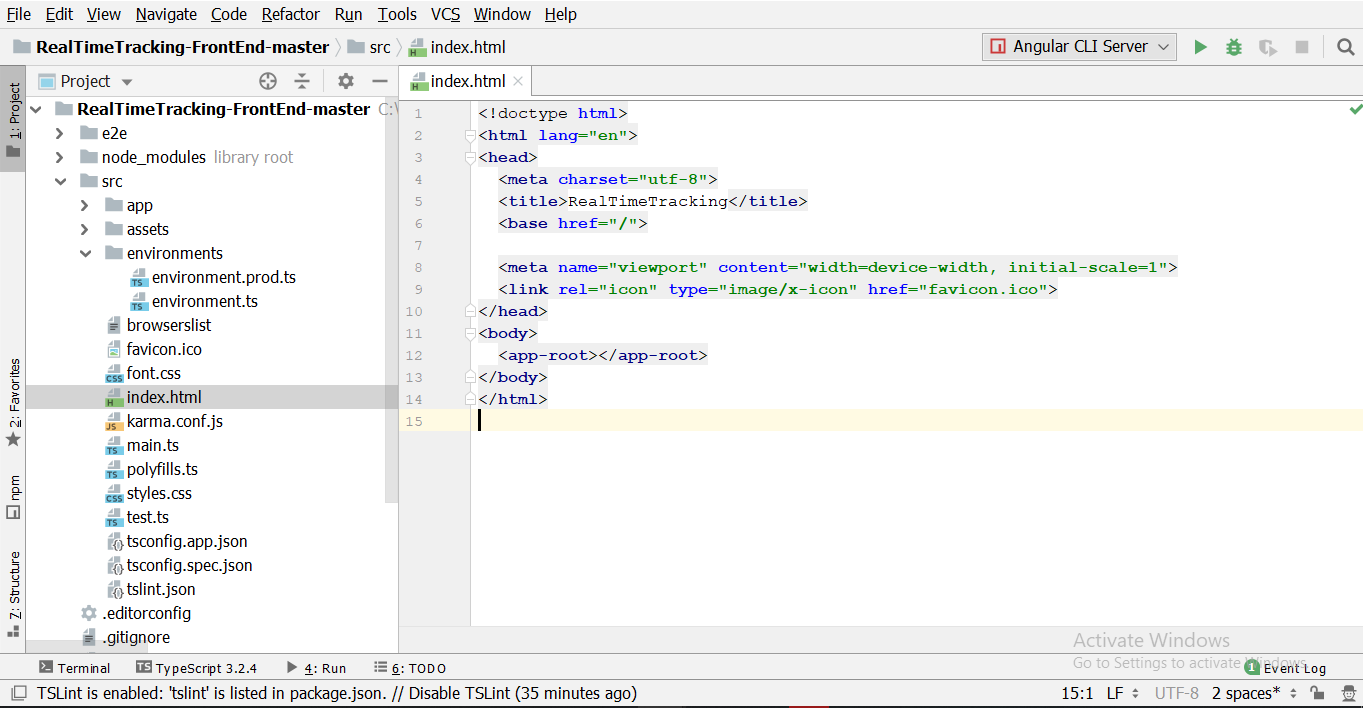
\includegraphics[width=1.1\textwidth]{code19}}
	\end{figure}
\end{enumerate}
                      
%--------------------------------------------------------------------------dictionary(واژه نامه ها)
%اگر مایل به داشتن صفحه واژه‌نامه نیستید، خط زیر را غیر فعال کنید.
%\parindent=0pt
%%
\chapter*{واژه‌نامه‌ی فارسی به انگلیسی}
\pagestyle{style9}

\addcontentsline{toc}{chapter}{واژه‌نامه‌ی فارسی به انگلیسی}
%%%%%%
\begin{multicols*}{2}

{\bf آ}
\vspace*{3mm}


\farsiTOenglish{اسکالر}{Scalar}


\vspace*{3mm}
{\bf ب}
\vspace*{3mm}

\farsiTOenglish{بالابر}{Lift}


\vspace*{3mm}
{\bf پ}
%%\vspace*{3mm}

\farsiTOenglish{پایا}{Invariant}



\vspace*{3mm}
{\bf ت}
%%\vspace*{3mm}

\farsiTOenglish{ تناظر }{Correspondence}


\vspace*{3mm}
{\bf ث}
%%\vspace*{3mm}

\farsiTOenglish{ثابت‌ساز}{Stabilizer}

\vspace*{3mm}
{\bf ج}
%%\vspace*{3mm}

\farsiTOenglish{جایگشت}{Permutation}



\vspace*{3mm}
{\bf چ}
%%\vspace*{3mm}


\farsiTOenglish{چند جمله‌ای }{Polynomial}

\vspace*{3mm}
{\bf ح}
%%\vspace*{3mm}

\farsiTOenglish{حاصل‌ضرب دکارتی}{Cartesian product}


\vspace*{3mm}
{\bf خ}
%%\vspace*{3mm}

\farsiTOenglish{خودریختی}{Automorphism}

\vspace*{3mm}
{\bf د}
%%\vspace*{3mm}

\farsiTOenglish{درجه}{Degree}


\vspace*{3mm}
{\bf ر}
%%\vspace*{3mm}


\farsiTOenglish{ریزپردازنده}{microprocessor}


\vspace*{3mm}
{\bf ز}
%%\vspace*{3mm}


\farsiTOenglish{زیرمدول}{Submodule}


\vspace*{3mm}
{\bf س}
%%\vspace*{3mm}

\farsiTOenglish{سرشت}{Character}


\vspace*{3mm}
{\bf ص}
%%\vspace*{3mm}

\farsiTOenglish{صادقانه}{Faithful}

\vspace*{3mm}
{\bf ض}
%%\vspace*{3mm}

\farsiTOenglish{ضرب داخلی}{Inner product}

\vspace*{3mm}
{\bf ط}
%%\vspace*{3mm}


\farsiTOenglish{طوقه}{Loop}


\vspace*{3mm}
{\bf ظ}
%%\vspace*{3mm}


\farsiTOenglish{ظرفیت}{Valency}
 
\vspace*{3mm}
{\bf ع}
%%\vspace*{3mm}


\farsiTOenglish{عدم مجاورت}{Nonadjacency}



\vspace*{3mm}
{\bf ف}
%%\vspace*{3mm}

\farsiTOenglish{فضای برداری}{Vector space}



\vspace*{3mm}
{\bf ک}
%%\vspace*{3mm}

\farsiTOenglish{کاملاً تحویل‌پذیر}{Complete reducibility}


\vspace*{3mm}
{\bf گ}
%%\vspace*{3mm}


\farsiTOenglish{گراف}{Graph}



\vspace*{3mm}
{\bf م}
%%\vspace*{3mm}

\farsiTOenglish{ماتریس جایگشتی}{Permutation matrix }


\vspace*{3mm}
{\bf ن}
%%\vspace*{3mm}

\farsiTOenglish{ناهمبند}{Disconnected}


\vspace*{3mm}
{\bf و}
%%\vspace*{3mm}

\farsiTOenglish{وارون‌پذیر}{Invertible}


\vspace*{3mm}
{\bf ه}
%%\vspace*{3mm}

\farsiTOenglish{همبند}{Connected}



\vspace*{3mm}
{\bf ی}
%%\vspace*{3mm}

\farsiTOenglish{یال}{Edge}




\end{multicols*}%
%%%%%%%
\chapter*{ واژه‌نامه‌ی انگلیسی به فارسی}
\pagestyle{style9}
\lhead{\thepage}\rhead{واژه‌نامه‌ی انگلیسی به فارسی}
\addcontentsline{toc}{chapter}{واژه‌نامه‌ی انگلیسی به فارسی}

\LTRmulticolcolumns
\begin{multicols}{2}
{\hfill\bf  \lr{A}}
%%\vspace*{1.5mm}

\englishTOfarsi{Automorphism}{خودریختی}

\vspace*{3mm}
{\hfill\bf   \lr{B}}
%%\vspace*{1.5mm}

\englishTOfarsi{Bijection}{دوسویی}

\vspace*{3mm}
{\hfill\bf   \lr{C}}
%%\vspace*{1.5mm}

\englishTOfarsi{Cycle group}{گروه دوری}

\vspace*{3mm}
{\hfill\bf   \lr{D}}
%%\vspace*{1.5mm}

\englishTOfarsi{Degree}{درجه}

\vspace*{3mm}
{\hfill\bf   \lr{E}}
%%\vspace*{1.5mm}

\englishTOfarsi{Edge}{یال}

\vspace*{3mm}
{\hfill\bf   \lr{F}}
%%\vspace*{1.5mm}

\englishTOfarsi{Function}{تابع}

\vspace*{3mm}
{\hfill\bf   \lr{G}}
%%\vspace*{1.5mm}

\englishTOfarsi{Group}{گروه}

\vspace*{3mm}
{\hfill\bf   \lr{H}}
%%\vspace*{1.5mm}

\englishTOfarsi{Homomorphism}{همریختی}

\vspace*{3mm}
{\hfill\bf   \lr{I}}
%%\vspace*{1.5mm}

\englishTOfarsi{Invariant}{پایا}

\vspace*{3mm}
{\hfill\bf   \lr{L}}
%%\vspace*{1.5mm}

\englishTOfarsi{Lift}{بالابر}

\vspace*{3mm}
{\hfill\bf   \lr{M}}
%%\vspace*{1.5mm}

\englishTOfarsi{Module}{مدول}

\vspace*{3mm}
{\hfill\bf   \lr{N}}
%%\vspace*{1.5mm}

\englishTOfarsi{Natural map}{نگاشت طبیعی}

\vspace*{3mm}
{\hfill\bf   \lr{O}}
%%\vspace*{1.5mm}

\englishTOfarsi{One to One}{یک به یک}

\vspace*{3mm}
{\hfill\bf   \lr{P}}
%%\vspace*{1.5mm}

\englishTOfarsi{Permutation group}{گروه جایگشتی}

\vspace*{3mm}
{\hfill\bf   \lr{Q}}
%%\vspace*{1.5mm}

\englishTOfarsi{Quotient graph}{گراف خارج‌قسمتی}

 \vspace*{3mm}
{\hfill\bf   \lr{R}}
%%\vspace*{1.5mm}

\englishTOfarsi{Reducible}{تحویل پذیر}

\vspace*{3mm}
{\hfill\bf   \lr{S}}
%%\vspace*{1.5mm}

\englishTOfarsi{Sequence}{دنباله}

 \vspace*{3mm}
{\hfill\bf   \lr{T}}
%%\vspace*{1.5mm}

\englishTOfarsi{Trivial character}{سرشت بدیهی}

\vspace*{3mm}
{\hfill\bf   \lr{U}}
%%\vspace*{1.5mm}

\englishTOfarsi{Unique}{منحصربفرد}

\vspace*{3mm}
{\hfill\bf   \lr{V}}
%%\vspace*{1.5mm}

\englishTOfarsi{Vector space}{فضای برداری}
\end{multicols}
%--------------------------------------------------------------------------index(نمایه)
%اگر مایل به داشتن صفحه نمایه نیستید، خط زیر را غیر فعال کنید.
\pagestyle{style7}
\printindex
\pagestyle{style7}
%کلمات کلیدی انگلیسی
\latinkeywords{Internet of Things, Real-Time Tracking System, SIM808, GPS, GSM}
%چکیده انگلیسی

\en-abstract{
	In the science of information technology, the concept of the Internet of objects refers to objects with a specific identity that have a unique identifier and the ability to transfer data to the network without the need for interaction and human intervention. In fact, its main purpose is to intelligent objects and provide a way through which objects can send and receive information with each other.\\
	In recents years, the technology of the Internet of Things has grown dramatically and has been able to meet various and complex needs in various fields. One of the Internet uses of objects is the tracking of moving objects that can be used in various areas, such as security, monitoring, transport, and so on.
	The positioning and tracking system offers the possibility of providing reliable solutions for the safety of individuals and vehicles, and also has a significant impact on the quality of the monitoring and management of transport fleets, the movement of vehicles, people (children and the elderly), or Each movable object has another. It is actually a technology tracking system that allows you to accurately locate and trace individuals, vehicles, or any other moving object using a variety of methods, such as the Global Positioning System.\\	
	This project presents the development of the remote vehicle
	tracking system which integrates the Global System for Mobile
	Communications (GSM) Modem and Google Map. we plan to implement a system that can be used to determine the precise position, direction, and locations of any moving object at any time.\\ In this system, each object is equipped with one that receives its location every two minutes from the satellite and sends it to the software servers via the modem of the GPS module. After downloading the software, the software servers analyze them as GSM. In this part of the project, a web application will be developed to process and sent information and then store it in a database, and finally convert the stored information to be displayed to users. This way, you can see the speed, the path, and the location of the object on the map.
}
%%%%%%%%%%%%%%%%%%%%% کدهای زیر را تغییر ندهید.

\newpage
\thispagestyle{empty}
\begin{latin}
\section*{\LARGE\centering Abstract}

\een-abstract

\vspace*{.5cm}
{\large\textbf{Key Words:}}\par
\vspace*{.5cm}
\elatinkeywords
\end{latin}
% در این فایل، عنوان پایان‌نامه، مشخصات خود و چکیده پایان‌نامه را به انگلیسی، وارد کنید.
%%%%%%%%%%%%%%%%%%%%%%%%%%%%%%%%%%%%
\baselineskip=.6cm
\begin{latin}

\latinfaculty{Department of ...}


\latintitle{Title of Thesis}


\firstlatinsupervisor{Dr. }

%\secondlatinsupervisor{Second Supervisor}

\firstlatinadvisor{Dr. }

%\secondlatinadvisor{Second Advisor}

\latinname{Name}

\latinsurname{Surname}

\latinthesisdate{Month \& Year}

\latinvtitle
\end{latin}

\end{document}